% \documentclass[11pt,twoside]{eitExjobb}
\documentclass[11pt,twoside,final]{eitExjobb}  % Use final for the final version that will be printed
%%%%%%%%%%%%%%%%%%%%%%%%%%%%%%%%%%%%%%%%%%%%%%%%%%%%
%% Other fonts (Palatino as rm font, helvetica as sf font and courier as tt font. All fonts are normally installed with a standard LaTeX distribution.)
% \usepackage{mathpazo} % Also in math mode
% \usepackage[scaled=.95]{helvet}
% \usepackage{courier}
%%%%%%%%%%%%%%%%%%%%%%%%%%%%%
%
\usepackage[utf8]{inputenc}  % Input encoding (this file): 8 bit unicode.
\usepackage[T1]{fontenc}     % Output encoding (pdf file)
%%%%%%%%%%%%%%%%%%%%%%%%%%%%%
%% Packages used
\usepackage{graphicx}   % Included graphics and some resizable boxes
\usepackage{url}        % nice urls with line breaks 
\usepackage{lipsum}     % nonsense text blocks
\usepackage{booktabs}   % nicer table rules
\usepackage[version=4]{mhchem}   % fancy chemical notation
\usepackage{siunitx}    % better unit notation
\DeclareSIUnit{\torr}{Torr}
\usepackage{fancyref}   % improved labels
\usepackage{parskip}    % better paragraph splitting
\usepackage{subcaption} % easier labeling of subfigures
\usepackage{floatrow}   % for setting table fontsize
%%%%%%%%%%%%%%%%%%%%%%%%%%%%%%
\patchcmd{\thebibliography}{\section*{\refname}}{}{}{}

\DeclareFloatFont{small}{\small}
\floatsetup[table]{font=small}
\floatsetup[table]{style=plaintop}
%%%%%%%%%%%%%%%%%%%%%%%%%%%%%%
%%%%%%%%%%%%%%%%%%%%%%%%%%%%%%
\begin{document}
%%% Title page
\Title{Flashlamp Annealing for Improved Ferroelectric Junctions}
\Author{Theodor Blom\\\texttt{nat13tbl@student.lu.se}}
\Supervisor{Mattias Borg}
\CoSupervisor{Rainer Timm}
\Examiner{Mathieu Gisselbrecht}
\Info{12 months, 60 hp}
%% Set by default
\Date{December 12, 2022}    %% Today's date
% \Year{\the\year} %% This year shown in copyright
% \Company{Department of Electrical and Information Technology\\Lund University}
%%%%%%
\MakeTitlePage{}  %%% Print title page and copyright page
%%%%%% 
\frontmatter    %%% Page numbering for front pages (small roman)
%%%%% Abstract
\chapter*{Abstract}
The effects of flashlamp annealing (FLA) on the quality of ferroelectric
\ce{Hf_xZr_{1-x}O2} (HZO) interfaces, integrated on \ce{InAs} substrates, are
evaluated. For the integration of ferroelectric HZO on III-V semiconductors the
crystallization via rapid thermal processing (RTP) can severely degrade the
HZO/III-V interface. Thermal annealing in the millisecond duration were used in
the efforts of reducing diffusion through the HZO film and increase device
performance. Electrical characterization showed a lower defect density and
improved endurance of the FLA samples compared to the RTP counterparts. The use
of multiple low-energy flashes and pre-crystallization during ALD growth was
also investigated for further improvement on device performance. Overall, this
work provides valuable insight into low thermal budget integration of HZO on
III-V semiconductors.

%%%%% Popular Science Summary
\chapter*{Popular Science Summary}
\subsection*{A New Frontier of Computing}
We all recognize the feeling of panic when your computer crashes and you realize
you forgot to save your progress for the past couple of hours. In this scenario
you wait for the computer to boot again and assess what you have lost. Imagine
instead the computer booting instantly and you find yourself exactly where you
left off. With an emerging technology in computer design this could become the
new reality.

The basic idea behind the fundamental building block of your electronic devices,
known as the transistor, has since its invention in the 1960s been largely
unchanged. The design which proved most successful is known as the
Metal-Oxide-Semiconductor Field Effect Transistor (MOSFET) and is by far the
most common design even to this day due to its cheap manufacturing process and
its ability to be scaled down to ever smaller devices. However, in the last
decade one has started to reach the limits of the MOSFET design, primarily due
to limited scalability, and alternative designs are actively being explored.

A promising design is the Ferroelectric Tunnel Junction (FTJ) which utilizes the
small dimensions of the transistor to its advantage where electrons tunnel
through a thin barrier. This barrier is then manipulated to either allow
electrons though or not, resulting in the characteristic transistor
functionality. In addition to being intrinsically small, the ferroelectric
barrier allows the transistor to be toggleable where the state of the transistor
is maintained even though power is lost. This ability means that electronic
devices utilizing this design does not have to be booted up, as all transistors
are already set to the desired state. Additionally, as power is only consumed as
transistors are being toggled between states, these devices could reduce power
consumption lengthening the battery life across all devices.

However, for this to become the new reality of computers, the FTJ design must be
improved further to prove as an effective alternative to the MOSFET design. One
limiting factor is believed to be the interfaces of the ferroelectric barrier
layer. Utilizing a new technique known as Flash-Lamp Annealing (FLA) the
processing of the ferroelectric barrier layer can be made up to 10 000 times
faster which could significantly improve the interfaces. This as the material
can set much faster resulting in better defined interfaces. If successful, this
could be a crucial step for this new transistor design to become a viable
alternative to MOSFETs and bring in a new frontier of computing.

%%%%% Preface
\chapter*{Self-reflection and Acknowledgements}
Before you is a masters thesis performed and (mostly) written during a
pandemic. When the project started in January 2021 there was continuous talk
about the reopening only being a couple of weeks ahead and towards the end me
and my supervisor were both surprised that we'd only met in person twice during
the full year. Luckily, the lab was still available and after an intense spring
of equipment training and method teachings I was ready to start fabricate and
characterize ferroelectric capacitors on my own. Many long days and a couple of
destroyed \ce{InAs}-substrates later all data was collected and visualized and
the process of putting words to my actions ensued. In this process I noticed a
mistake, I found myself re-reading many of the articles I had read during the
spring to find the sources to back my claims. I should have found a reliable
process and started indexing my sources earlier. In the end this set me back
and in late November 2021 I realized I would not be able to finish writing the
thesis before the December deadline. This also hindered me from dedicating
enough time to polishing the figures in the result section. Furthermore, a
special year for Lund was in the works with a coming Lundakarneval which ended
up taking more of my attention than I anticipated. A year later in December
2022 I wrote the final sentence of this thesis now in your possession.

I wish to give special thanks to my supervisor Mattias Borg for his insights
and guidance throughout the project as well as his patience in me finishing
this thesis. This would not have been possible without our weekly checkups,
even though they were done through a computer screen.\\
I also wish to thank Robin Athle for teaching me the laboratory equipment and
the methods used in this thesis. Thanks for making yourself available for
questions big and small and being an inspiration to keep pushing further.

%% ToC etc
\tableofcontents
\listoffigures
\listoftables
\cleardoublepage{}
%%%%% Page numbering for the main thesis (arabic)
\mainmatter{}
%%%%%%%%%%%%%%%%%%%%%%%%%%%%
\chapter{Introduction}\label{ch:intro}

The integration of electronic devices in our daily lives hardly goes unnoticed.
Chances are that you are reading this very paper on an electronic device;
either your phone, your computer or even your watch. To keep up with demand a
lot of research is being conducted on designing faster, smaller and more energy
efficient devices. A step in this direction is improving upon the basic
building block of all devices, the transistor.

The transistor is the physical component which is toggled between ones (on) and
zeroes (off) in order to store and process digital information. A common design
of the transistor is the so called metal-oxide-semiconductor
field-effect-transistor (MOSFET) where the application of a voltage to a metal gate
electrode is used to control the current through the semiconductor channel of the
transistor. This classic design has been steadily improved for decades but has
in recent years reached a performance plateau primarily due to scaling
difficulties \cite{ratnech2021advancement}.

As the MOSFET decreases in size, the effects of electron tunneling increase and
eventually the difference in current between the on and off state becomes
indistinguishable rendering the device useless. In 1971 it was theorized and
proposed that one could develop a transistor which uses the tunneling
characteristics of the electron as the source of the switching current. The
concept was dubbed Ferroelectric Tunneling Junctions (FTJs) but was dismissed
and forgotten as ferroelectric materials was not believed to work on smaller
structures. From there the use of ferroelectric materials in transistor
development was kept to a very small niche of specific applications where
scalability of the devices were not an issue and can be found on the market
today as FeRAMs and FeFETs with a junction length of >\SI{100}{\nano\meter}
\cite{garcia2014ferroelectric, mikolajick2020past}.

This was all changed in 2011 when Böscke et.al. published a paper revealing the
successful creation of a \SI{10}{\nano\meter} ferroelectric tunneling junction
\cite{boscke2011ferroelectricity}. They used lightly doped hafnium oxide
(\ce{HfO2}) which was crystallized to a ferroelectric phase. A truly remarkable
discovery which reignited a lot of interest in ferroelectric materials for
transistor design. Ferroelectric transistors have the advantage of being
non-volatile which means they can be read without having to restore the state
of the transistor (rewrite). This reduces the energy consumption dramatically
and could be a key factor in reducing the overall energy consumption of all
digital devices. Additionally, the discovery of ferroelectric hafnium oxide is
of great importance as \ce{HfO2} already is a common material in modern transistor
manufacturing. This allows for a simplified integration of ferroelectric
transistors in current device designs \cite{mikolajick2020past}.

Ferroelectric tunneling junctions using hafnium oxide has previously been
demonstrated. In 2020 a \SI{1}{\nano\meter} ferroelectric thin-film was
integrated on \ce{Si} and in 2021 a \SI{10}{\nano\meter} junction was
integrated on \ce{InAs} \cite{cheema2020one, athle2021effects}. However, a
common denominator of these devices is a limited endurance. A modern MOSFET
should be able to perform at least $10^{12}$ cycles before degradation but FTJs
of today are usually only cycled roughly $10^6$ cycles before breakdown. This
can be amended with techniques such as junction bilayers and reduced cycling
voltage but one crucial limiting factor is the thermal stresses endured by the
device in the crystallization process.

To reduce the thermal stresses one would need to minimize the time and
temperature of the crystallization process, also known as the thermal budget.
In 2018 it was demonstrated that it was possible to achieve similar performing
FTJs using the fast crystallization technique of Flashlamp Annealing (FLA) to
the commonly used crystallization technique of Rapid Thermal Processing (RTP) 
\cite{oconnor2018stabilization}. The reduction of the thermal budget on the
devices is not only preferred for the performance of the individual transistor
but also crucial for the successful integration into current device designs.
Using nanosecond laser annealing, the integration of a FTJ in a production
environment was demonstrated in 2020. Their devices showed significantly
improved endurance over previous efforts \cite{grenouillet2020nanosecond}.

These efforts show the capability of FTJs as integrated on \ce{Si} and metal
electrodes. Integration of FTJs on III-V semiconductors have not been studied
in as much detail. Specifically, the integration of FTJs on \ce{InAs} provide
new challenges due to the diffusion and oxygen affinity of both \ce{In} and
\ce{As} \cite{kang2016structural}. This paper demonstrates the improved
performance of FTJs as integrated on \ce{InAs} using the FLA technique compared
to RTP.
    
%%%%%%%%%%%%%%%%%%%%%%%%%%%
\chapter{Ferroelectric Junctions}\label{ch:ferro}

\section{Ferroelectricity}\label{sec:ferro}

Ferroelectric materials have the property of retaining an internal electric
field even after an external electric field is removed
\cite{dawber2005physics}. The ferroelectric nature of the material is not
uniform but rather comprised of many small-scale fields that can be aligned
from an external source in order to propagate and strengthen the field
throughout the material. In the case of ferroelectric materials the small-scale
fields are referred to as domains where each domain has its own electric field
strength and direction in 3D-space. The domains are separated by domain walls
of varying thickness where the field is rapidly and repeatedly changing between
the domain field directions. The domain boundaries can arise from electrical
and thermal treatment of the samples but are mostly determined by the
spontaneously oriented fields of the domains \cite{damjanovic2006hysteresis}.

The amount of alignment between domains of a ferroelectric material is denoted
its polarization and is often measured in
\si{\micro\coulomb\per\centi\meter\squared}. As a ferroelectric material is
created the spontaneously polarized domains are unaligned and the ferroelectric
nature of the material is obscured. However, by applying an external electric
field over the material the domains rotate to align with the external source.
As the external source is removed the aligned domains remain and hence also the
built-in electric field. The polarization remaining after the removal of the
external electric field is called the remnant polarization. The sequence of
polarizing is illustrated in figure \ref{fig:theo_domain}.

\begin{figure}[htbp]
    \centering
    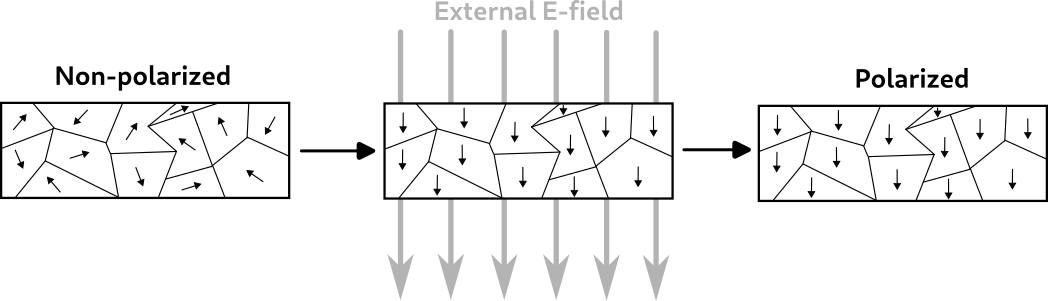
\includegraphics[width=0.80\textwidth]{fig/img/polarized.png}
    \caption{Schematic figure of the process of domain alignment to an external
    electric field. Initially the domains are spontaneously polarized to
    different polarization directions but with the application of an external
    electric field the domains are aligned and the ferroelectric material is
    polarized.}
    \label{fig:theo_domain}
\end{figure}

The domains are typically not uniform and may require different external field
strength in order to "wakeup" and align themselves with the external field. The
required external field strength to polarize a ferroelectric sample is referred
to as the coercive field and is often measured in
\si{\mega\volt\per\centi\meter}. The quantitative definition of the coercive
field is described in figure \ref{fig:theo_PE} but is commonly illustrated
using the energy landscape as in figure \ref{fig:theo_Ec}. Here the
polarization of the ferroelectric sample is in a binary system where the
application of an external electric field allows for the polarization to
"topple over" to the other polarization direction when the external electric
field is stronger than the coercive field of the sample.

\begin{figure}[htbp]
    \centering
    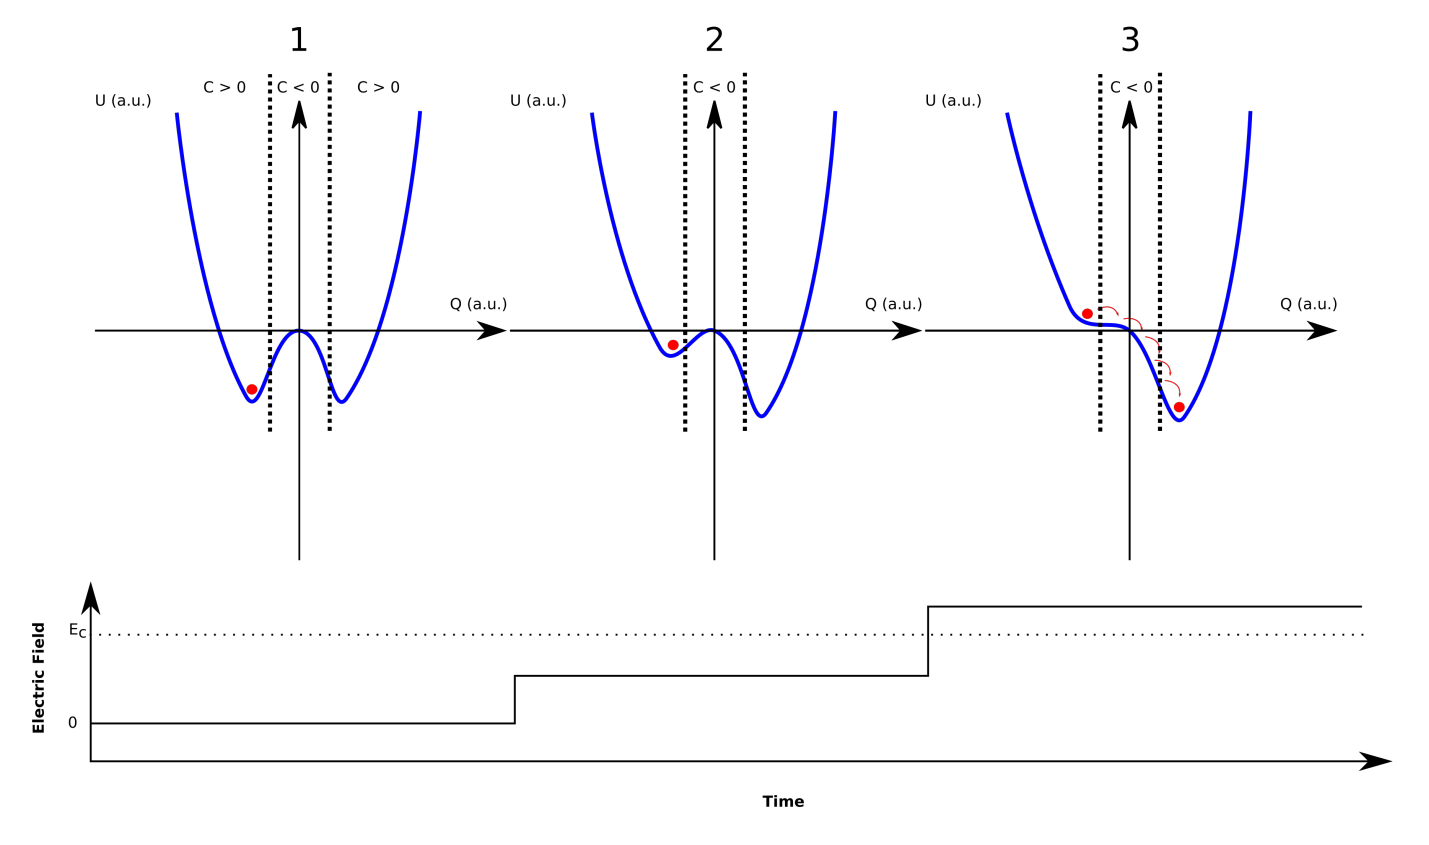
\includegraphics[width=0.95\textwidth]{fig/img/coercivefield.png}
    \caption{Energy landscape of a ferroelectric material through the
    polarization event. In the absence of an external electric field the
    polarization state is bound to its current trough. But with the application
    of a small electric field the potential between the barriers are lowered until
    the field if eventually greater than the coercive field $E_c$ and the
    polarization of the material is switched. Figure taken from R. Athle
    \cite{athle2019development}.}
    \label{fig:theo_Ec}
\end{figure}

These two properties, remnant polarization ($P_r$) and coercive field ($E_c$),
form the basis of how ferroelectric materials are characterized. These
properties are best illustrated through a P-E curve which relates the
polarization of a ferroelectric film with the electric field strength applied
over the film. For a non-ferroelectric material the P-E curve would show a
linear relationship between the two. However, for a ferroelectric material clear
hysteresis is observed as the polarization remains with electric field
strength approaching zero. An illustration of a P-E curve is shown in figure
\ref{fig:theo_PE}. The polarization is initially set to applying an external
electric field ($E$) following the green dashed line. However, as the external
field is reduced to zero the hysteresis of the ferroelectric material is
revealed. Once polarized, the polarization remains without the influence of an
external field ($P_r^+$). In order to switch the polarization, an opposite
external electric field stronger than the coercive field of the
material ($E_c^-$) must be applied. Removing the external field again shows
that the polarization indeed has been switched. Important to note is that it is
not possible to measure the absolute polarization of the ferroelectric
materials, only the change of it as the polarization is measured through the
current in the switching event.

\begin{figure}[htbp]
    \centering
    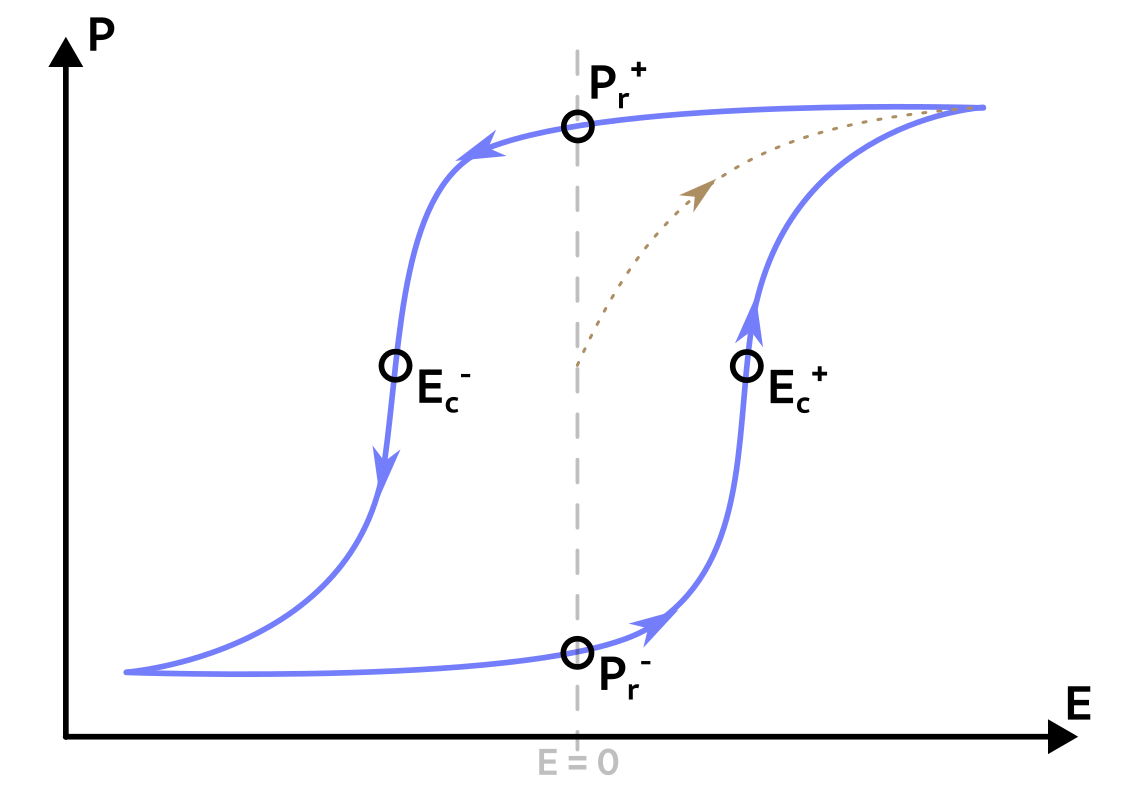
\includegraphics[width=0.60\textwidth]{fig/img/PE.png}
    \caption{Schematic graph of a P-E curve showing the two properties of a
        ferroelectric material; the remnant polarization ($P_r$) and the
        coercive field ($E_c$).}
    \label{fig:theo_PE}
\end{figure}

\subsection{\ce{HfZrO2}}

Ferroelectric materials were first conceptualized in the 1950s along with the
boom of the computing era. However, one quickly encountered integration and
scalability issues with the ferroelectric materials of the time and the concept
was soon forgotten to the well known MOSFET architecture
\cite{mikolajick2020past}. In 2011 the field of ferroelectrics was revived with
the discovery of ferroelectric \ce{HfO2}. Hafnium oxide was and is a commonly
used oxide in integrated circuits today and could hence overcome the previous
integration issues \cite{boscke2011ferroelectricity}. An intermediary
orthorhombic phase (O) was theorized between the then known stable,
non-ferroelectric amorphous (A) and monoclinic phases (M). The orthorhombic
phase is non-centrosymmetric enabling the ferroelectric polarization behaviour
to be retained by the material. With the addition of \ce{ZrO2} of varying
composition ranges the ferroelectric, orthorhombic phase of \ce{HfO2} was more
easily stabilized and was later proved to be scalable overcoming even the
second hurdle 60 years prior \cite{muller2012ferroelectricity, cheema2020one}.

The orthorhombic phase of \ce{HfZrO2} (HZO) is reached through annealing and is
highly dependant on both film composition as well as time and temperature of the
annealing step. The equal distribution of \ce{Hf_{0.5}Zr_{0.5}O2} is known to
be the optimal choice for both stability and ferroelectric response
\cite{muller2012ferroelectricity}. A thorough investigation of the phase
transformations of HZO in 2019 showed the transformation from the orthorhombic
to the monoclinic phase requiring a volume expansion. Capping the amorphous
film before annealing is hence a big step in suppressing the $O \rightarrow M$
transformation \cite{migita2019phase}. Despite our best efforts, HZO grains of
both the amorphous and monoclinic phases will most likely remain in the sample
but maximizing the volume fraction of the orthorhombic phase is possible.

\section{The FTJ Structure and Operation}

The concept of the Ferroelectric Tunnel Junction (FTJ) was first proposed in 1971
but as the integration and scalability issues of ferroelectric materials of the
time was not solved the concept was forgotten as thin films was essential for
the functionality. The FTJ concept is based on using the polarization state to
control the tunneling of electrons through the ferroelectric barrier. Because
of the ferroelectric charges, the electrostatic potential of the barriers
($\Phi$) is altered and is different depending on the polarization direction.
Figure \ref{fig:theo_FTJband} shows a band diagram of a metal-insulator-metal
(MIM) junction. Since the tunnel transmission depends exponentially on the
square root of the barrier height, the current through the barrier will be
dependant on the direction of the polarization \cite{garcia2014ferroelectric}. 

\begin{figure}[htbp]
    \centering
    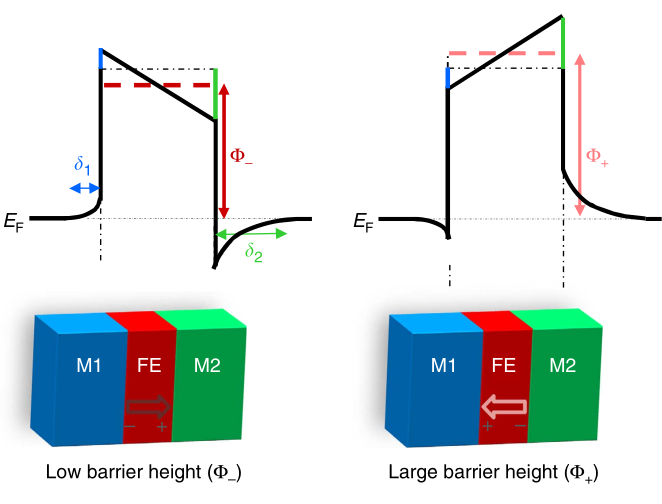
\includegraphics[width=0.55\textwidth]{fig/img/FTJbandstructure.png}
    \caption{Band structure of a MIM FTJ. The asymmetry between the two
        electrodes allows for different electrostatic potential ($\Phi$)
        depending on the polarization direction. The difference in potential
        allows for accurate control over the tunneling current through the
        barrier. Image taken from Garcia et.al. \cite{garcia2014ferroelectric}}
    \label{fig:theo_FTJband}
\end{figure}

For the electrostatic potential to be different between the two polarization
states the asymmetry between the two interfaces is essential. One way of
introducing asymmetry is integrating the ferroelectric onto a semiconductor
with a limited density of states. The use of ferroelectrics in integrated
circuits is limited but the FTJ concept was proven to work in 2020 using
\SI{1}{\nano\meter} HZO integrated onto \ce{Si} \cite{cheema2020one,
mikolajick2020past}. However, FTJ devices are yet to prove sufficiently good to
be considered for practical applications and thus further research is required
in improved annealing and integration on III-V semiconductors to fully realize
their potential.

\subsection{Leakage Mechanics and Defects}\label{sec:leakage}

A looming issue of the HZO-based ferroelectric tunnel junctions (FTJ) of today
is the increase of leakage current through the device with continued
polarization switching (cycling). This can be attributed to the generally
higher coercive field of HZO which causes high electrical field stress on the
devices, limiting endurance \cite{mikolajick2020past}. The high stresses of
cycling causes charge injection into existing vacancies which can either
facilitate or impede the ferroelectric response. This effect is known as
depinning and pinning of the domains respectively. In the pristine state,
some existing vacancies are charge injected which pins certain domains/grains
from participating in the switching event. Initial cycling allows for
the redistribution of vacancies and depinning of the domains to create a more
uniform field and allow for more domains to contribute to the polarization.
This is known as the wake-up-phase. However, further cycling generates
additional vacancies at the interfaces which screens the bulk of the
ferroelectric and makes it more difficult to reach the coercive field of all
domains. The generated vacancies can subsequently diffuse into the bulk
trapping charges which pins the domains from participating in the switching.
This is known as the fatigue phase of the ferroelectric. Further vacancy
generation collects at the grain boundaries of the HZO significantly increasing
the leakage current until breakdown of the device \cite{pesic2016physical}.
Figure \ref{fig:theo_pinning} shows an illustration of the pinning and
depinning of domains throughout cycling. Furthermore, a paper investigating the
structural properties of the integration of ferroelectric HZO on \ce{InAs} in
2016 showed the diffusion of both \ce{In} and \ce{As} atoms through the HZO
layer during annealing which significantly affects performance of the device
\cite{kang2016structural}.

Both of these effects are induced by the diffusion of defects throughout the
HZO. Diffusion is both temperature and time dependant so reducing the time the
sample is at an elevated temperature is paramount to reducing the effects of
these defects. This is known as the thermal budget of the sample. A common
fabrication technique of ferroelectric HZO is to crystallize the oxide in the
order of minutes called Rapid Thermal Annealing (RTP). By using other
techniques such as Flashlamp Annealing (FLA) or Pulsed-Laser Annealing (PLA)
are known techniques for reducing the thermal budget the samples are exposed
to \cite{oconnor2018stabilization, grenouillet2020nanosecond, volodina2021ferroelectric}.

\begin{figure}[htbp]
    \centering
    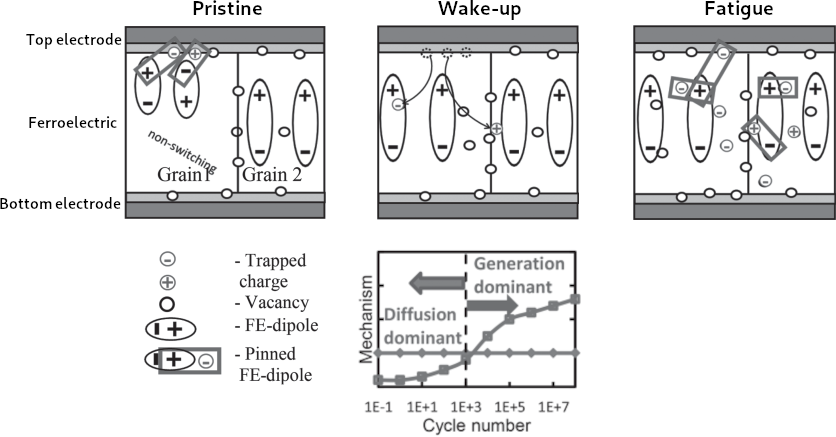
\includegraphics[width=0.85\textwidth]{fig/img/DomainPinning.png}
    \caption{Illustration of the (de-)pinning behavior throughout cycling and
        how the dominant defect mechanism changes from diffusion to generation
        for the device to enter the fatigue cycling phase. Image adapted from
        Pesic et.al. \cite{pesic2016physical}}
    \label{fig:theo_pinning}
\end{figure}
    

%%%%%%%%%%%%%%%%%%%%%%%%%%%
\chapter{Fabrication}\label{ch:fab}

Metal-Ferroelectric-Semiconductor capacitors with are to be fabricated using
traditional techniques. The MFS-caps were fabricated in a stack of
\ce{InAs}/\ce{HZO}/\ce{TiN} with an \ce{Au} contact on top. All fabrication was
done at Lund NanoLab (LNL) and is outlined in section \ref{sec:FabProc}. After
fabrication the resulting capacitors have the parameters as stated in table
\ref{tab:fab_param} and look like the picture in figure \ref{fig:fab_babycomp}.

\begin{table}[htbp]
    \centering
    \caption{Relevant fabrication parameters of the samples. Growth and
    annealing parameters of each sample is stated in Chapter
    \ref{ch:res}.}\label{tab:fab_param}
    \begin{tabular}{crc}
        \toprule
        Layer & Thickness & Doping \\\midrule
        \ce{Au} & \SI{200}{\nano\meter} & - \\ 
        \ce{TiN} & \SI{10}{\nano\meter} & - \\ 
        \ce{HfZrO2} & \SI{10}{\nano\meter} & 1:1 (\ce{Hf/Zr}) \\ 
        \ce{InAs} & \SI{280}{\micro\meter} &
        \SI{1e16}{\per\centi\meter\tothe{3}} \\\bottomrule 
    \end{tabular}
\end{table}

\begin{figure}[htbp]
    \centering
    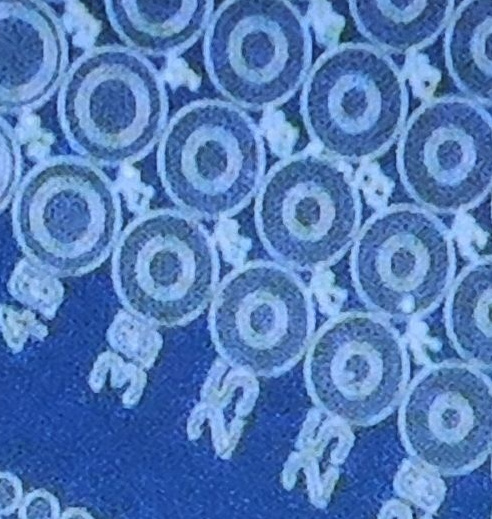
\includegraphics[width=.30\linewidth]{fig/img/babycomputers.jpg}
    \caption{Picture of fabricated capacitor rings. The numbering refers to the
    diameter of the inner capacitor circle in
    \si{\micro\meter}.}\label{fig:fab_babycomp}
\end{figure}

\section{Sample Fabrication Process}\label{sec:FabProc}

\subsection{InAs Wafer Preparation}
The initial substrate was a low doped \ce{InAs} \SI{4}{\inch} wafer with a
layer of \ce{In} and \ce{As} oxides on top. Since the wafer is to be used as
bottom contact of our capacitors a wet etch was required before any film
deposition was possible. The wafer was etched in 10:1 \ce{HCl} acid for
\SI{30}{\second} and rinsed in deionized \ce{H2O} to remove any oxides. The
samples were dried using a nitrogen gun and promptly advanced to the next step
to reduce reoxidation. This process is schematically showed in figure
\ref{fig:fab_1}. Before etching the wafers were cut into squares with a side
length of roughly \SI{10}{\milli\meter} to simplify processing.

\begin{figure}[htbp]
    \centering
    
\includegraphics[width=.70\linewidth]{fig/fabproc/fab_1.png}
    \caption{Schematic figure of the sample oxide etching process.}\label{fig:fab_1}
\end{figure}

\subsection{\ce{HfZrO2} Deposition}
With the native \ce{InAs} oxides removed the deposition of \ce{Hf_xZr_{1-x}O2}
was done using atomic layer deposition (ALD) in a Picosun Sunale R-100 system.
Samples were grown using alternating cycles (1:1) of TEMA(Hf) and TEMA(Zr)
precursors to achieve equal distribution of \ce{Hf} and \ce{Zr} ($x=0.5$) in
the resulting $\sim$\SI{10}{\nano\meter} oxide. Depending on the sample series
both chamber temperature and the number of cycles were altered. The specific
growth parameters for each samples is specified in Appendix \ref{app:procparam}.
Figure \ref{fig:fab_2} shows a schematic of the samples at this fabrication
stage.

\begin{figure}[htbp]
    \centering
    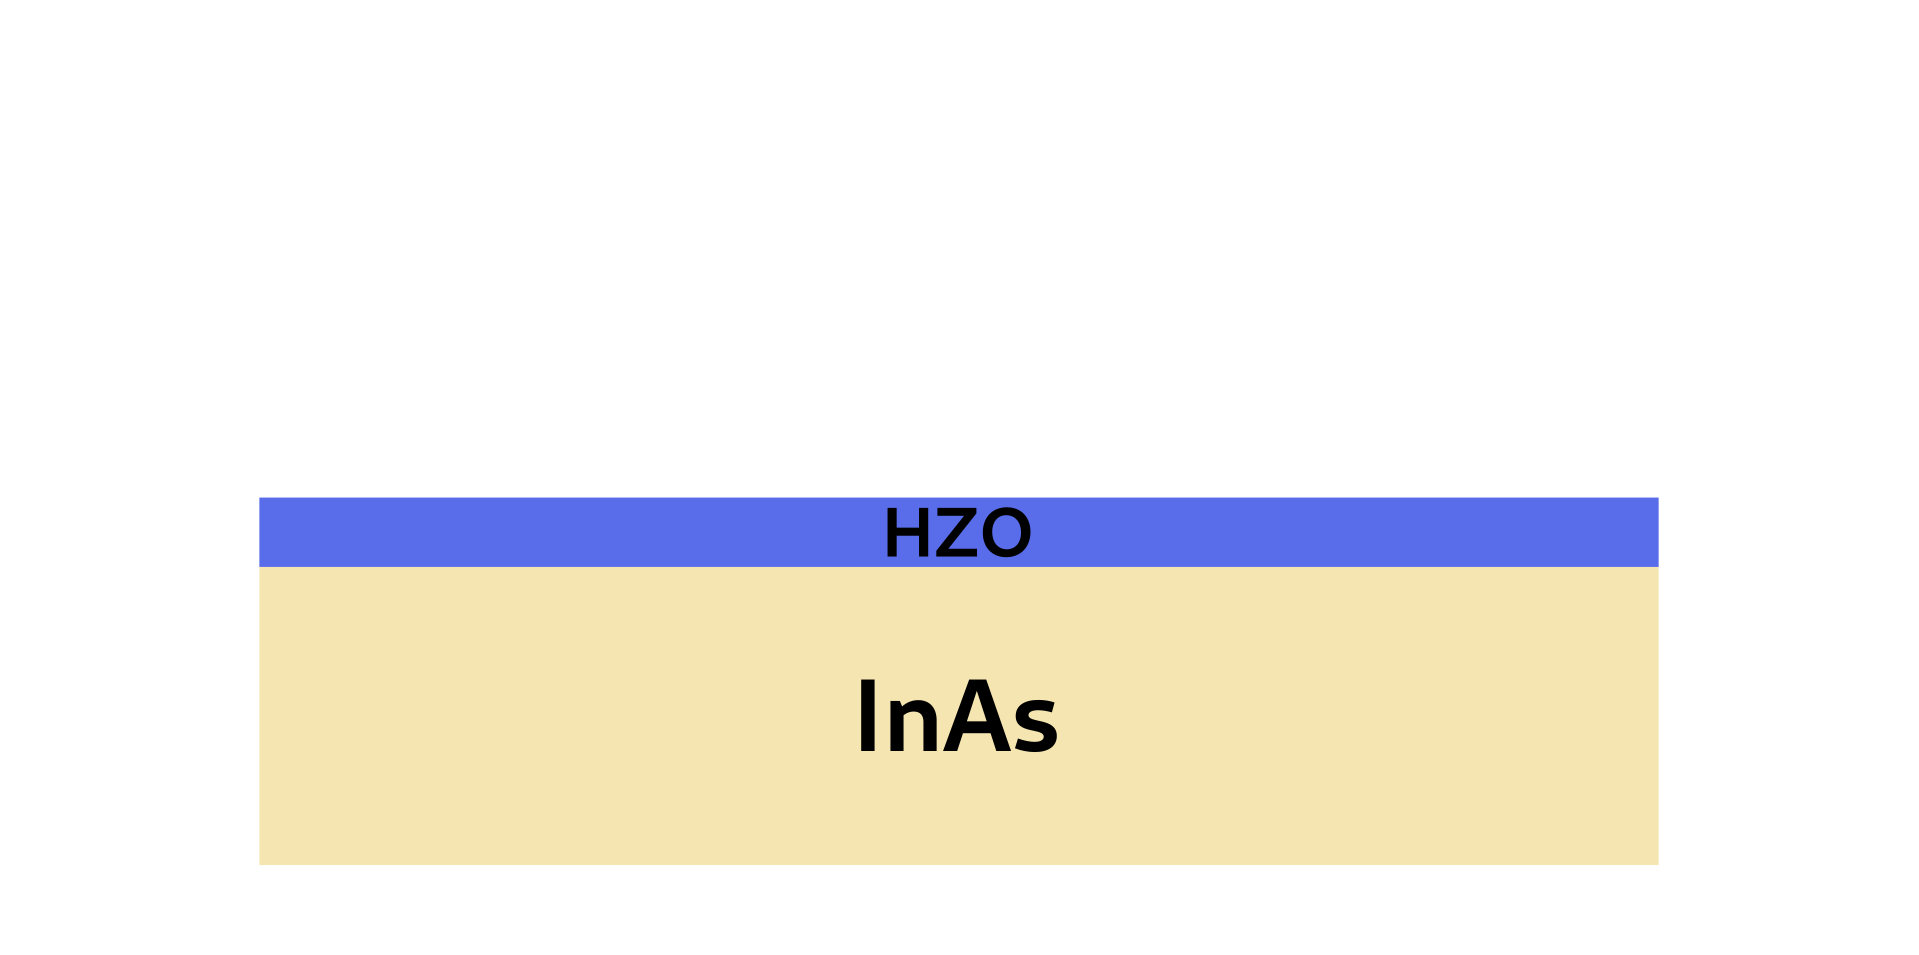
\includegraphics[width=.45\linewidth]{fig/fabproc/fab_2.png}
    \caption{Schematic figure of the sample after atomic layer
    deposition.}\label{fig:fab_2}
\end{figure}

\subsection{Top Electrode Deposition}
After deposition of the \ce{HfZrO2} film, a $\sim$\SI{10}{\nano\meter} top
contact of \ce{TiN} was deposited through sputtering using an AJA Orion 5
sputter machine. Pumping the chamber to <\SI{2.7}{\milli\torr} and pre-cleaning
the source for \SI{5}{\minute} the samples were sputtered at a power of
\SI{150}{\watt}. Sputtering for $\sim$\SI{11}{\minute} at a deposition rate of
\SI{0.15}{\nano\meter\per\second} resulted in the desired layer thickness.
Figure \ref{fig:fab_3} shows a schematic of the samples at this stage of
fabrication.

\begin{figure}[htbp]
    \centering
    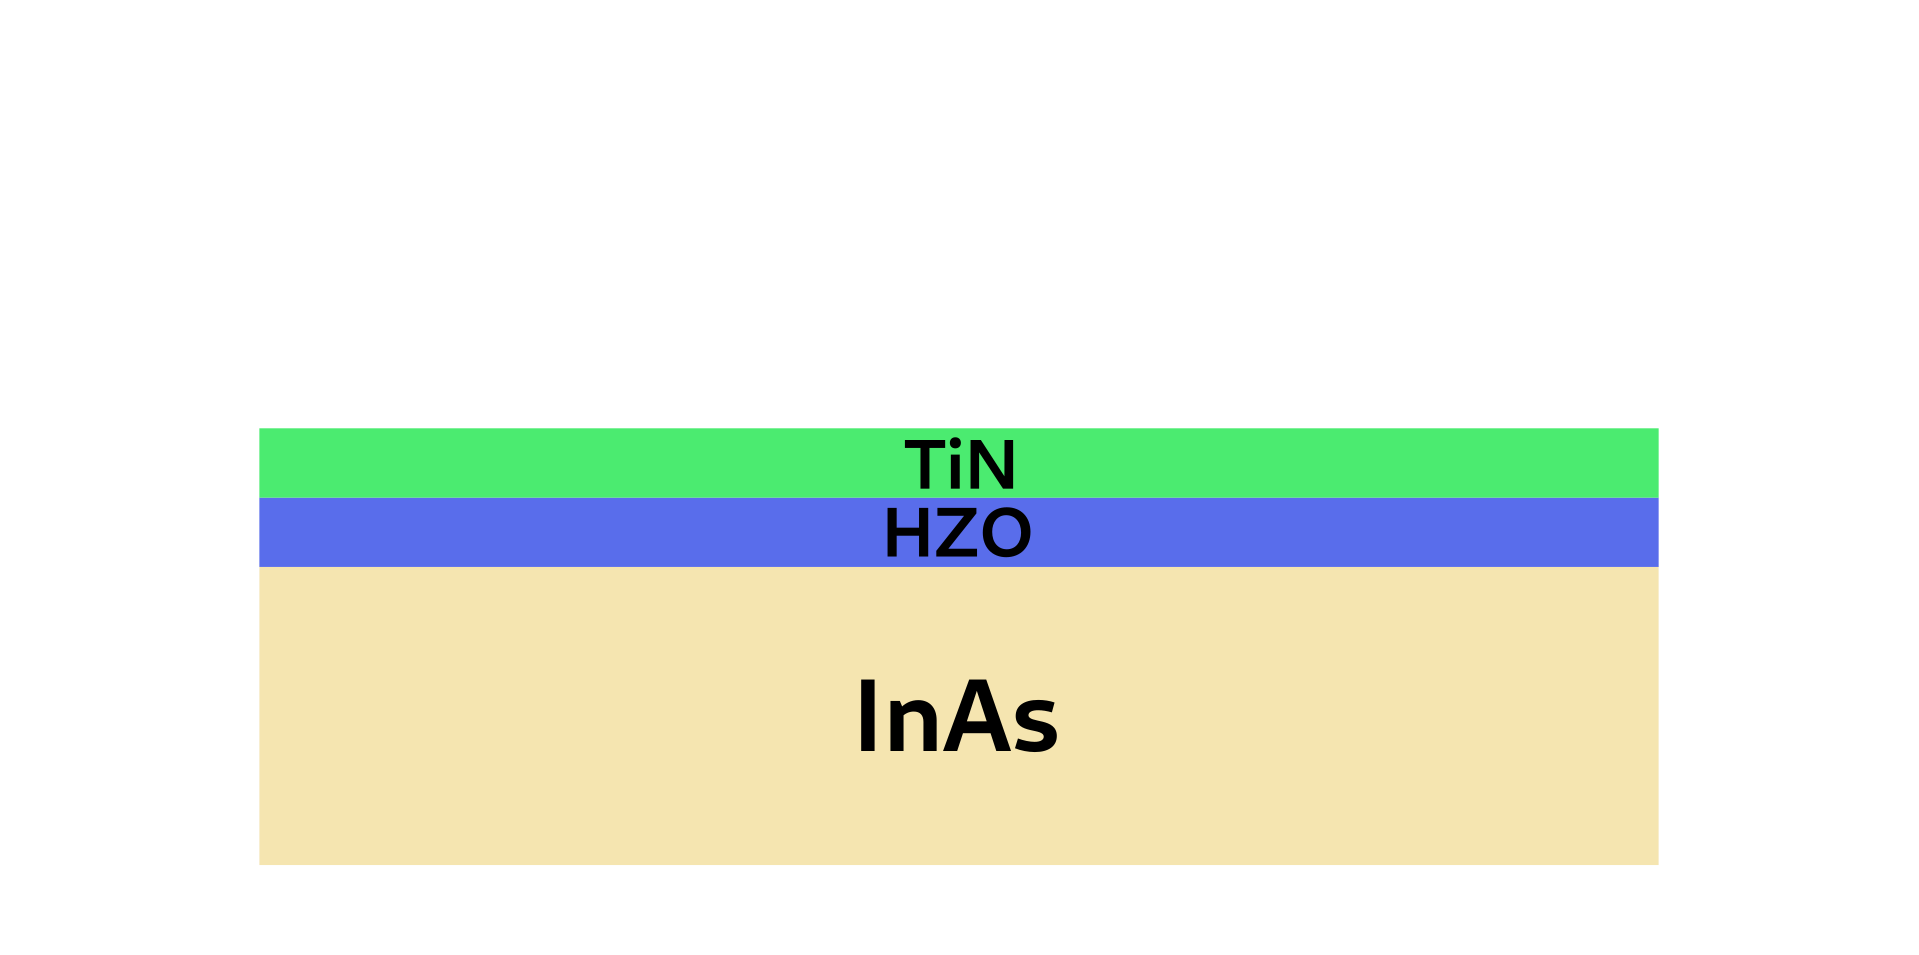
\includegraphics[width=.45\linewidth]{fig/fabproc/fab_3.png}
    \caption{Schematic figure of the sample after top contact
    sputtering.}\label{fig:fab_3}
\end{figure}

\subsection{Annealing Process}
With the amorphous oxide contained between the bottom- and the top contact annealing
could take place. Depending on the sample annealing was either done through
rapid thermal processing (RTP) or flash lamp annealing (FLA). The reference RTP
sample were annealed at \SI{600}{\celsius} for \SI{30}{\second} in a
RTP-1200-100 system from UniTemp GmbH while all other samples were annealed in
the FLA system by \SI{5}{\milli\second} pulses of varying energy and number.
See figure \ref{fig:res_Comsol} and Appendix \ref{app:procparam} for a detailed
overview of the number of flashes per sample and their energies. For the
interested reader an in-depth review of the FLA technique is available through
L. Rebohle et.al. \cite{rebohle2016review}.

\subsection{Metal Contacting}
In order to electrically characterize the samples, individual devices would
have to be defined as well as covered in thicker highly conductive \ce{Au} to
not damage the underlying structure using the probe techniques described in
Chapter \ref{ch:char}. The devices were defined using optical lithography and
the \ce{Au} was deposited using electron-beam evaporation. Figure
\ref{fig:fab_4} shows a schematic of the samples at this stage of fabrication.

\begin{figure}[htbp]
    \centering
    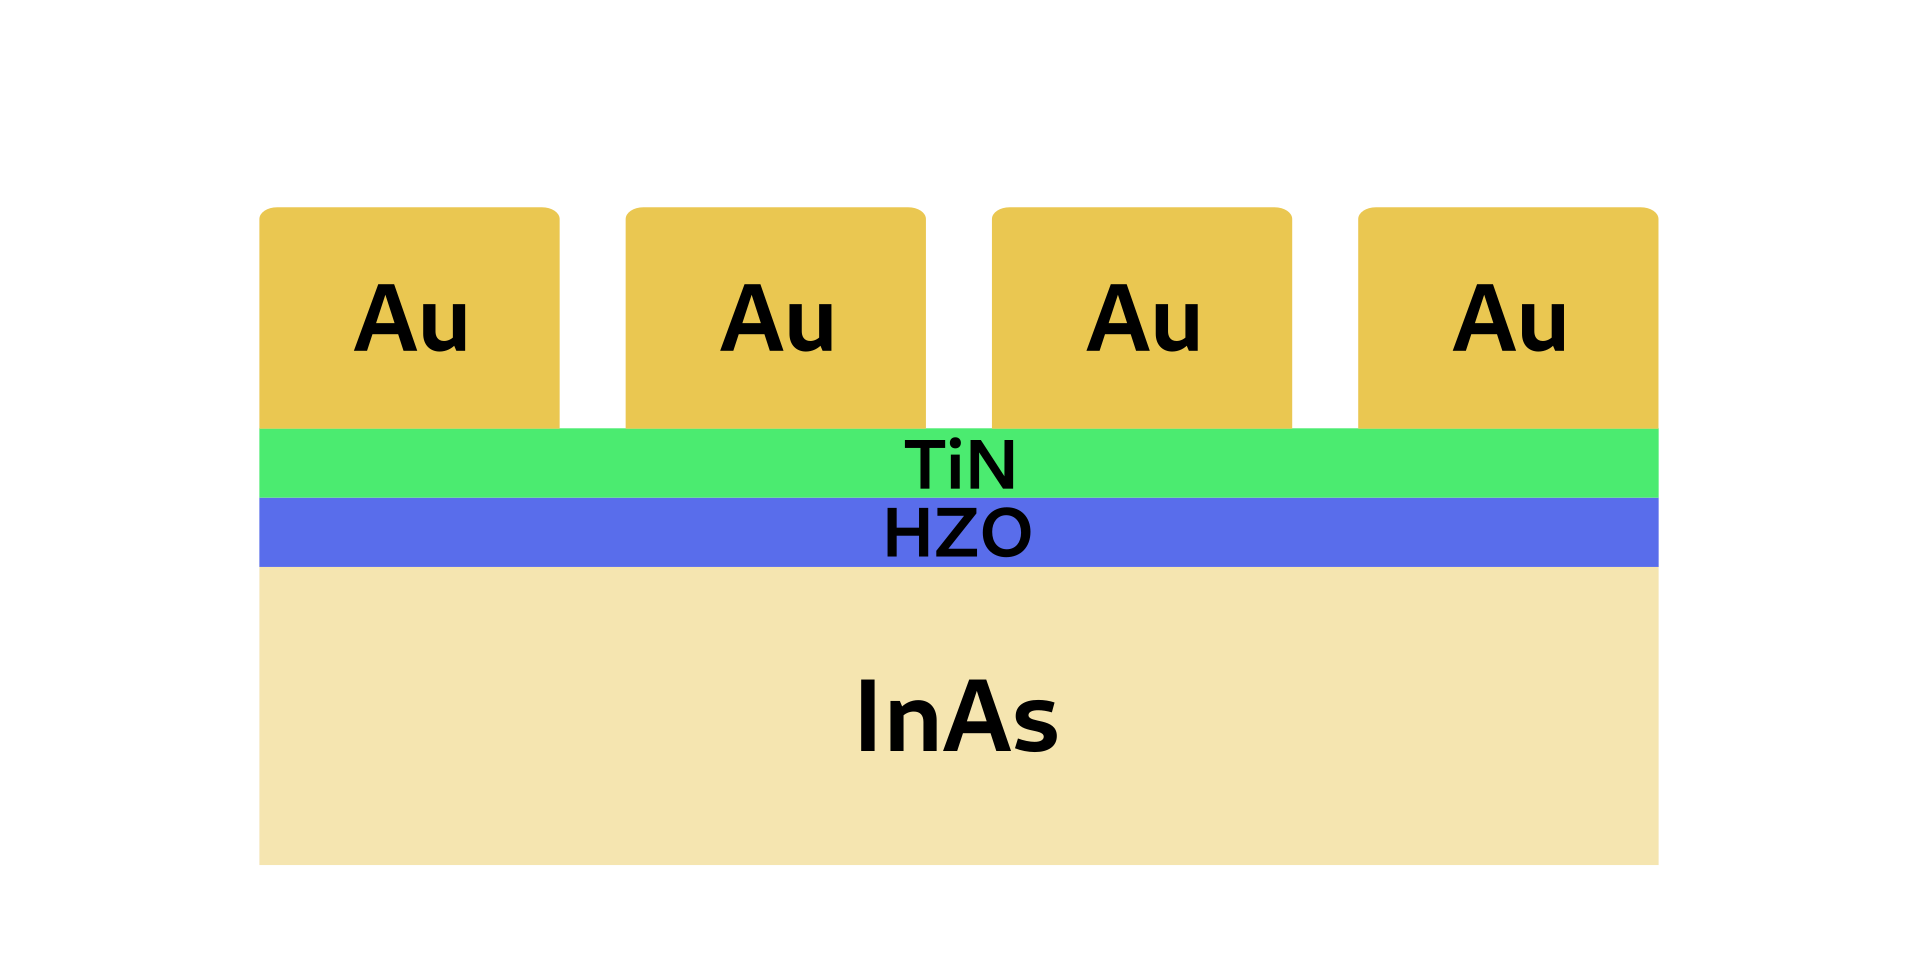
\includegraphics[width=.45\linewidth]{fig/fabproc/fab_4.png}
    \caption{Schematic figure of the sample after device definition and \ce{Au}
    deposition.}\label{fig:fab_4}
\end{figure}

\subsection{Etching of Top Contact}
To further define the devices the \ce{TiN} top contact was etched away in order
to avoid short circuiting. Using a wet-etch in \ce{NH4OH}:\ce{H2O2}:\ce{H2O} at
the ratio of 1:2:5 at \SI{60}{\celsius} the \ce{TiN} was selectively etched
away over a duration of \SI{30}{\second}. Maintaining the samples still in the
wet-etch hindered over-etching and ensured that there was no residue \ce{TiN}
short circuiting the capacitors. Figure \ref{fig:fab_5} shows a schematic of
the finished samples. See figure \ref{fig:fab_babycomp} for a picture of one of
the samples.

\begin{figure}[htbp]
    \centering
    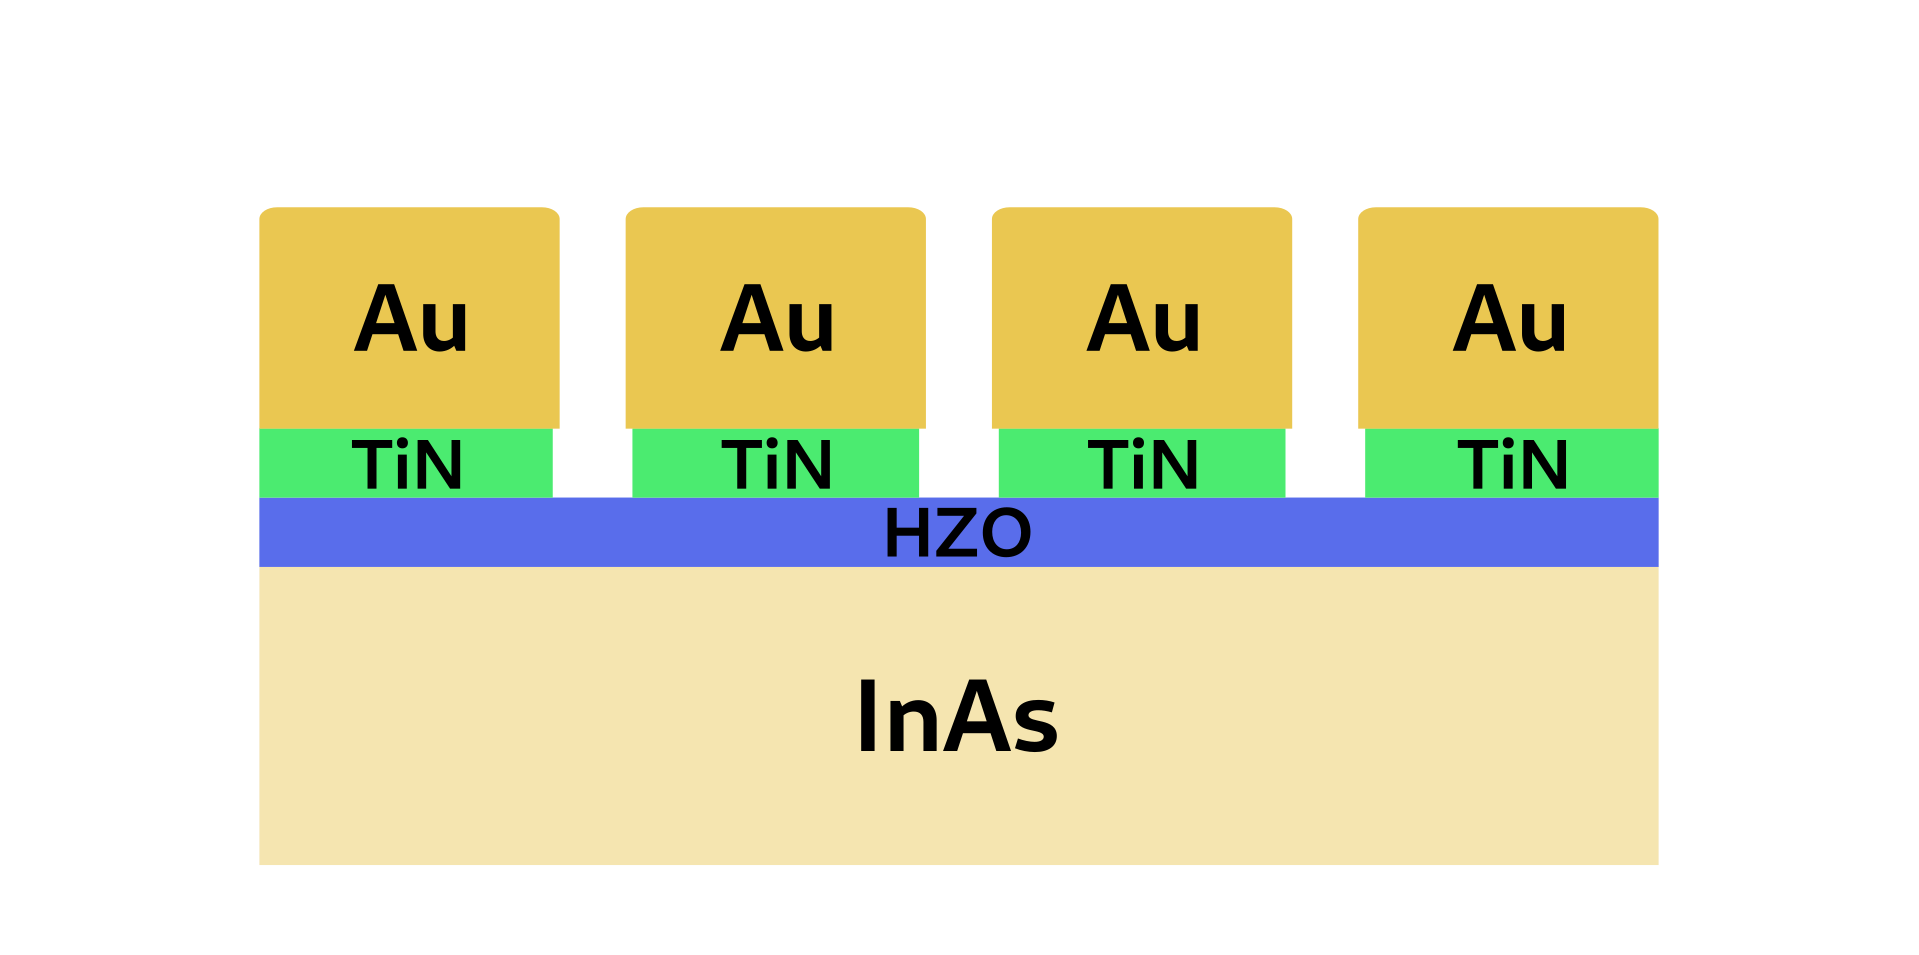
\includegraphics[width=.45\linewidth]{fig/fabproc/fab_5.png}
    \caption{Schematic figure of the sample after top contact etching. This is
    the finished sample.}\label{fig:fab_5}
\end{figure}

To summarize the chapter a step by step schematic of the entire fabrication
process can be seen in figure \ref{fig:fab_done}.

\begin{figure}[htbp]
    \centering
    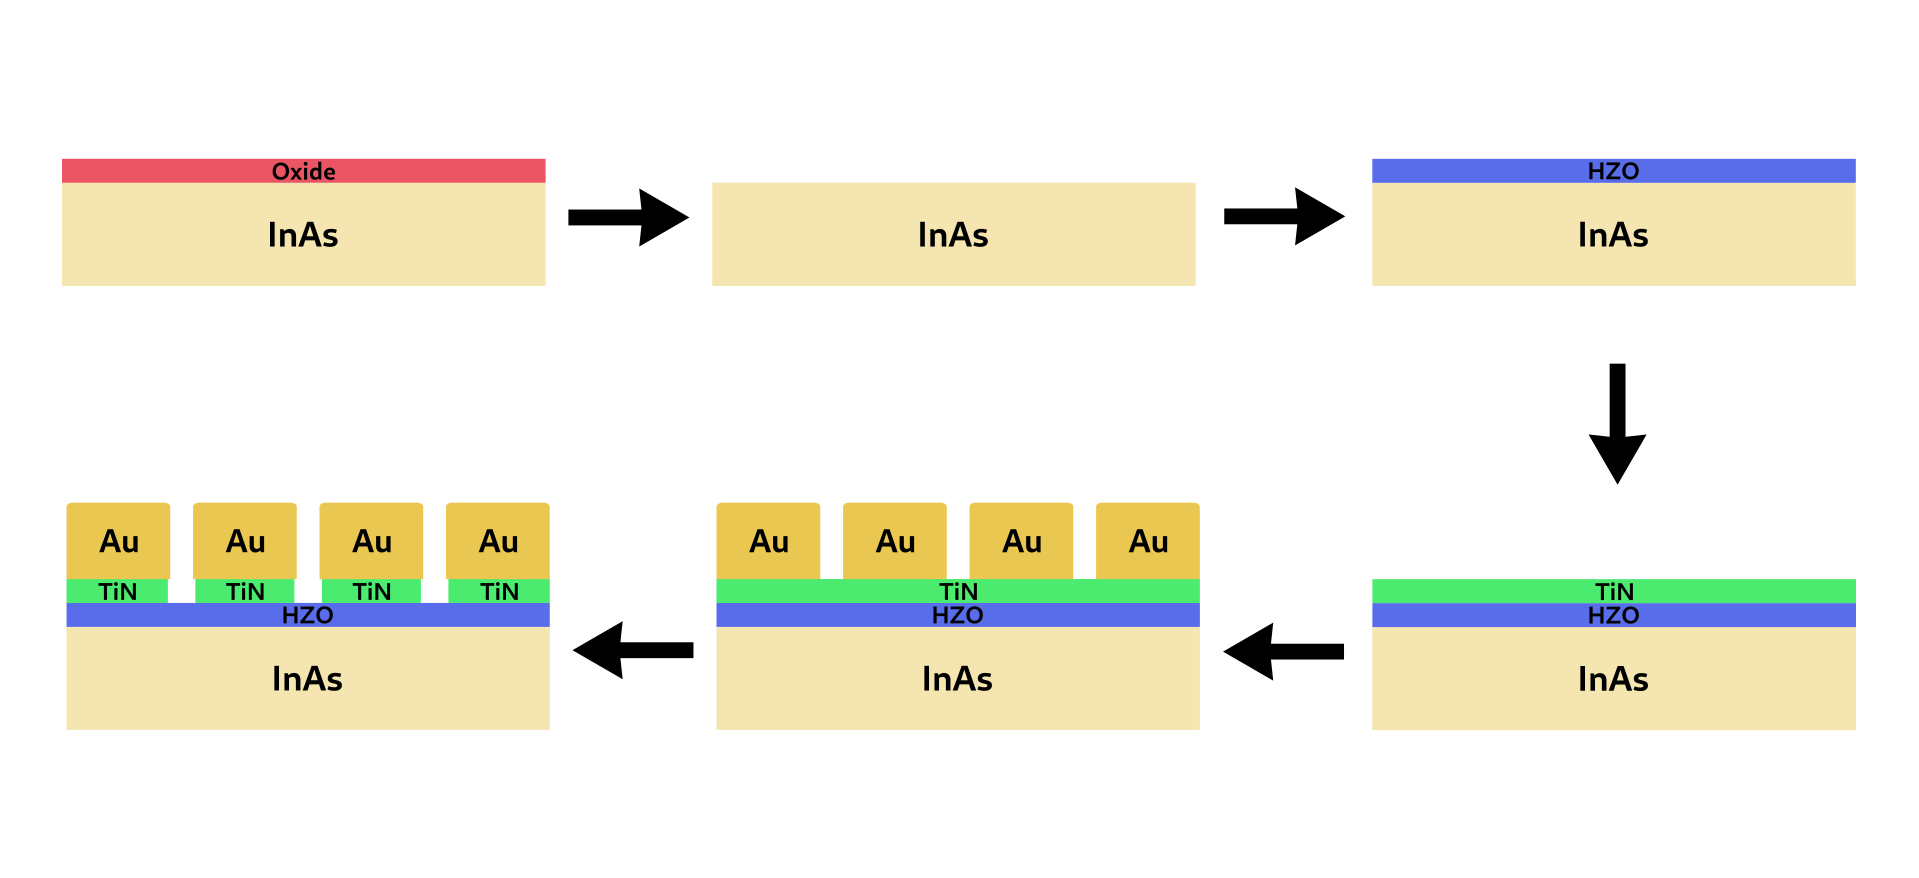
\includegraphics[width=.80\linewidth]{fig/fabproc/fab_done.png}
    \caption{Schematic figure of the entire fabrication process.}\label{fig:fab_done}
\end{figure}

%%%%%%%%%%%%%%%%%%%%%%%%%%
\chapter{Electrical Characterization}\label{ch:char}

To characterize the fabricated samples three different techniques were used;
Positive-Up-Negative-Down (PUND), endurance pulsing and a Capacitance-Voltage scheme to
quantitatively estimate the defect density of ferroelectric films integrated on
semiconductors. \cite{persson2020method} All characterization was done at the
Department of Electrical and Information Technology at Lund University.

\section{PUND and Endurance}\label{sec:PandE}
The PUND and endurance measurements of the samples were done simultaneously by
endurance pulsing up to $10^4$ cycles before conducting the PUND measurements to
later continue the endurance pulsing until breakdown of the sample. The two
methods are described individually in the following two sections. Both methods
werre performed using a Keysight B1500A parameter analyser equipped with a
B1530A waveform generator.

\subsection{PUND}\label{sec:PUND}
The Positive-Up-Negative-Down (PUND) method is used to quantitatively measure
the remnant polarization ($P_r$) and the coercive field ($E_c$) of a
ferroelectric device. These properties of ferroelectric films are explained in
Section \ref{sec:ferro}. The main goal of the technique is to remove the
influence of leakage current in the total current in order to determine the
amount of polarization current in the switching event.

\begin{figure}[htbp]
    \centering
    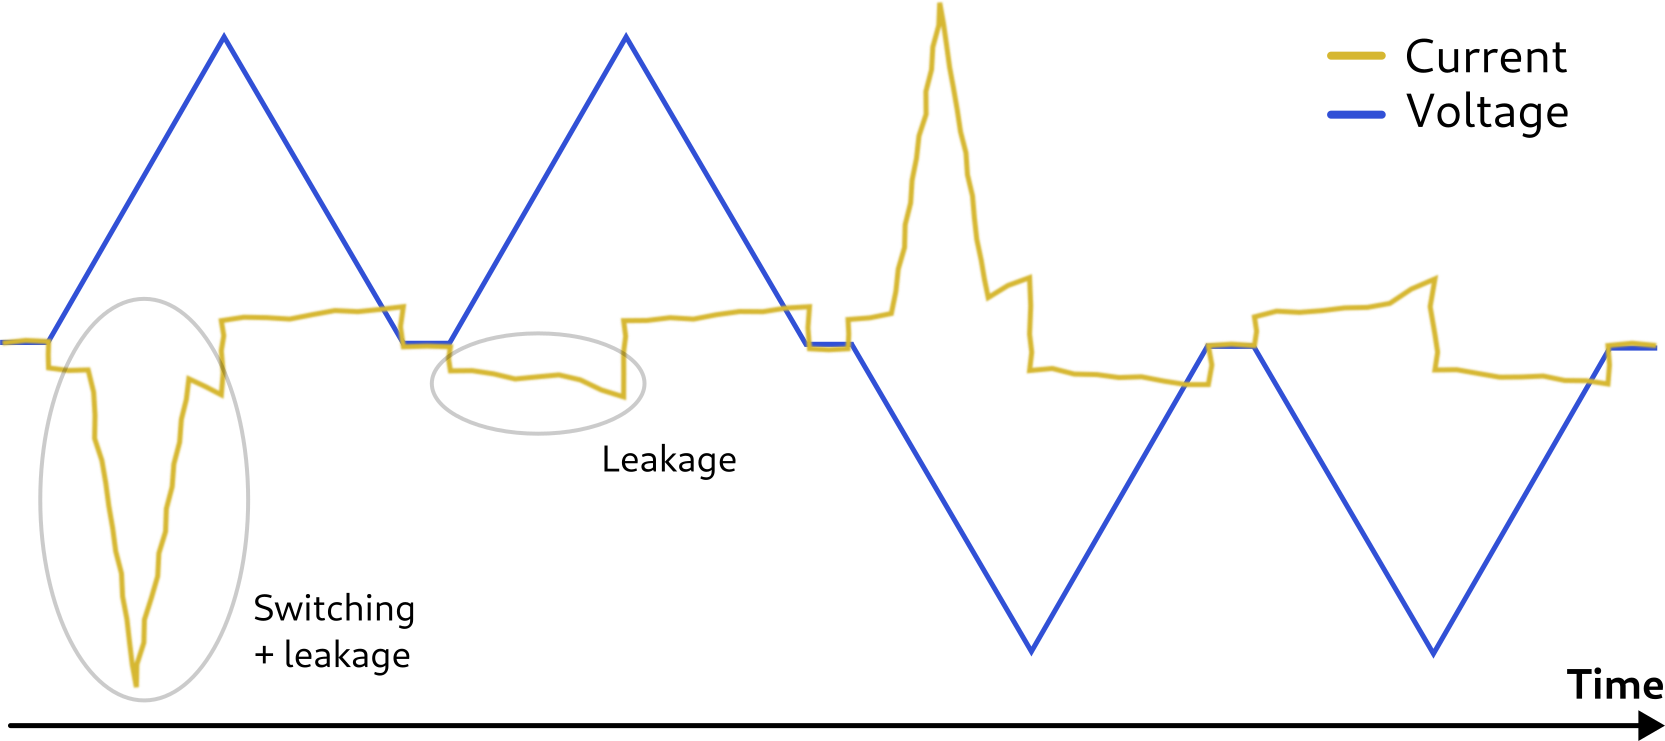
\includegraphics[width=0.70\textwidth]{fig/img/PUND.png}
    \caption{Schematic figure of a PUND measurement. The two consecutive
    voltage spikes only causes a ferroelectric switching event during the first
    spike which allows for the removal of the leakage current from the total
    current through integration.}
    \label{fig:char_PUND}
\end{figure}

Figure \ref{fig:char_PUND} illustrates the applied voltage and the current
response of the ferroelectric device. Four voltage spikes in the shape of
up-up-down-down are applied over the film. The first spike polarizes the film
towards the positive and gives a current response containing both the
polarization current as well as any leakage current. Since the polarization
field is already positive for the second spike only the leakage current is
measured. By removing the response of the second spike from the first one can
isolate the polarization current in the switching event. Repeating the same
idea for the negative-down pulses gives us the full name;
Positive-Up-Negative-Down.

Isolating the polarization current allows for better visualization of the
ferroelectric properties through the P-E curve described in Section
\ref{sec:ferro}. To achieve a graph as illustrated in Figure \ref{fig:theo_PE},
the applied voltage is scaled with the film thickness to achieve a unit of
electric field in \si{\mega\volt\per\centi\meter} and the polarization current
is time-integrated to obtain the accumulated polarization charge at each
electric field strength and scaled to the area of the device resulting in a
unit of \si{\micro\coulomb\per\centi\meter\squared}. From these data the
remnant polarization ($P_r$) and coercive field ($E_c$) of each device is
extracted.

\subsection{Endurance}\label{sec:Endu}
The endurance of a device is a measurement of how many cycles the device can
endure before polarization switching no longer can be measured. Polarization
switching induces more leakage through the device which eventually causes
breakdown as described in section \ref{sec:leakage}. By applying a voltage in a
sawtooth pattern over the ferroelectric film the device is rapidly switched
between the two polarization directions. Throughout cycling the electrical
response of the device is observed and cycling is stopped when breakdown
occurs. The number of cycles before breakdown is noted and assigned as the
endurance of the device.

\section{Capacitance-Voltage}\label{sec:CV}
Capacitance-Voltage (CV) measurements can be used to measure a multitude of
different properties. In this paper a specific CV measurement schema described
by A. E. Persson et.al. in 2020 was used to quantitatively estimate the amount
of defects in the ferroelectric films. \cite{persson2020method} The method is
based on the hysteresis of the CV curves induced by defects before the coercive
field is reached and the hysteresis is exaggerated by the switching current.
When the voltage on the device is swept up and down the band structure across
the film changes as illustrated in Figure \ref{fig:char_hysteresis}a and b
respectively. Sweeping towards the positive allows for electrons to flow from
the \ce{InAs} substrate into the oxide leading to a negative charge buildup at
the defect states of the oxide while the opposite is true for a bias sweep
towards the negative. This effect creates a shift of the bias voltage in the CV
measurement as shown by Figure \ref{fig:char_hysteresis}c. By Gauss' law, the
voltage shift $\Delta V_{th}$ and the charge density $Q_t q$ can be related by
equation \ref{eq:char_Vshift} where $C_{ox}$ is the oxide capacitance density,
$d$ is the oxide thickness and $\rho(x)$ is the defect charge density.

\begin{equation}\label{eq:char_Vshift}
    \Delta V_{th} = - \frac{1}{C_{ox}d} \int_0^d x\rho(x)\ \mathrm{d}x
    \Longrightarrow Q_t = \frac{\Delta V_{th}C_{ox}}{q}
\end{equation}

\begin{figure}[htbp]
    \centering
    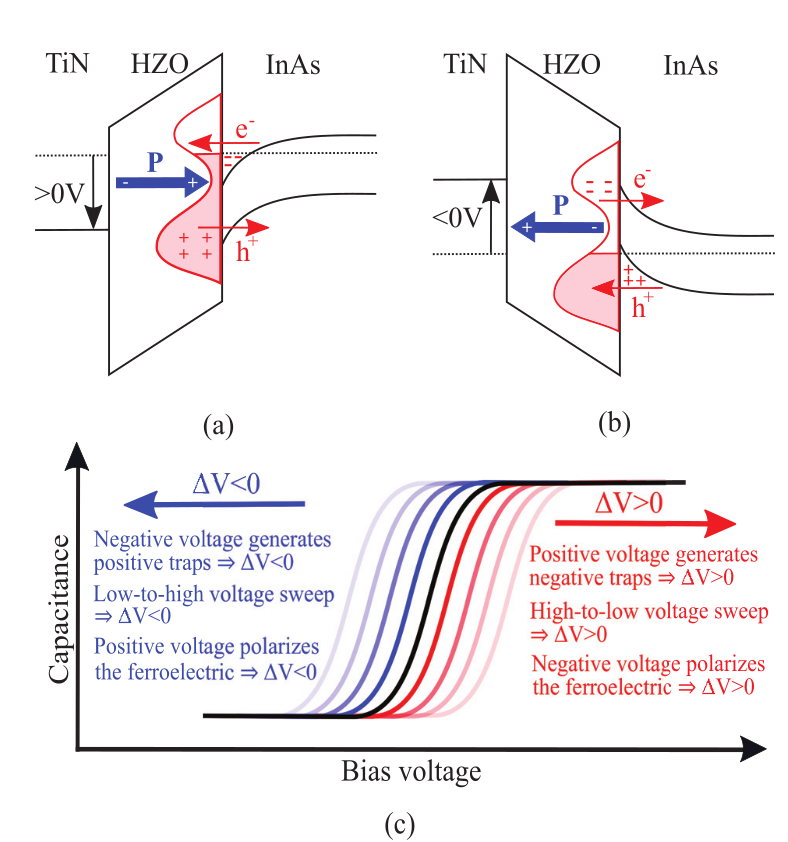
\includegraphics[width=0.65\textwidth]{fig/img/CV_hysteresis.png}
    \caption{The used CV method is based on charge trapping in the voltage
        sweeps. Figure a and b shows negative and positive charge buildup at
        the defect states in the oxide at a positive and negative voltage sweep
        respectively. The charge buildup in each case shifts the bias voltage
        towards the negative and positive respectively as described in figure
        c. The figure is borrowed from A. E. Persson et.al. \cite{persson2020method}}
    \label{fig:char_hysteresis}
\end{figure}

Equation \ref{eq:char_Vshift} allows for a quantization of the amount of
detected traps in the oxide $Q_t$ depending on the voltage shift $\Delta
V_{th}$ between the up and down voltage sweep. Figure \ref{fig:char_CV}
illustrates the measurement schema used to obtain $\Delta V_{th}$ and $C_{ox}$
for each device to calculate the defect density $Q_t$. Our measurements were
performed using a Agilent 4294A Impedence Analyser at a temperature of
\SI{13}{\kelvin} and a oscillation frequency and AC amplitude of
\SI{1}{\mega\hertz} and \SI{50}{\milli\volt} respectively.

\begin{figure}[htbp]
    \centering
    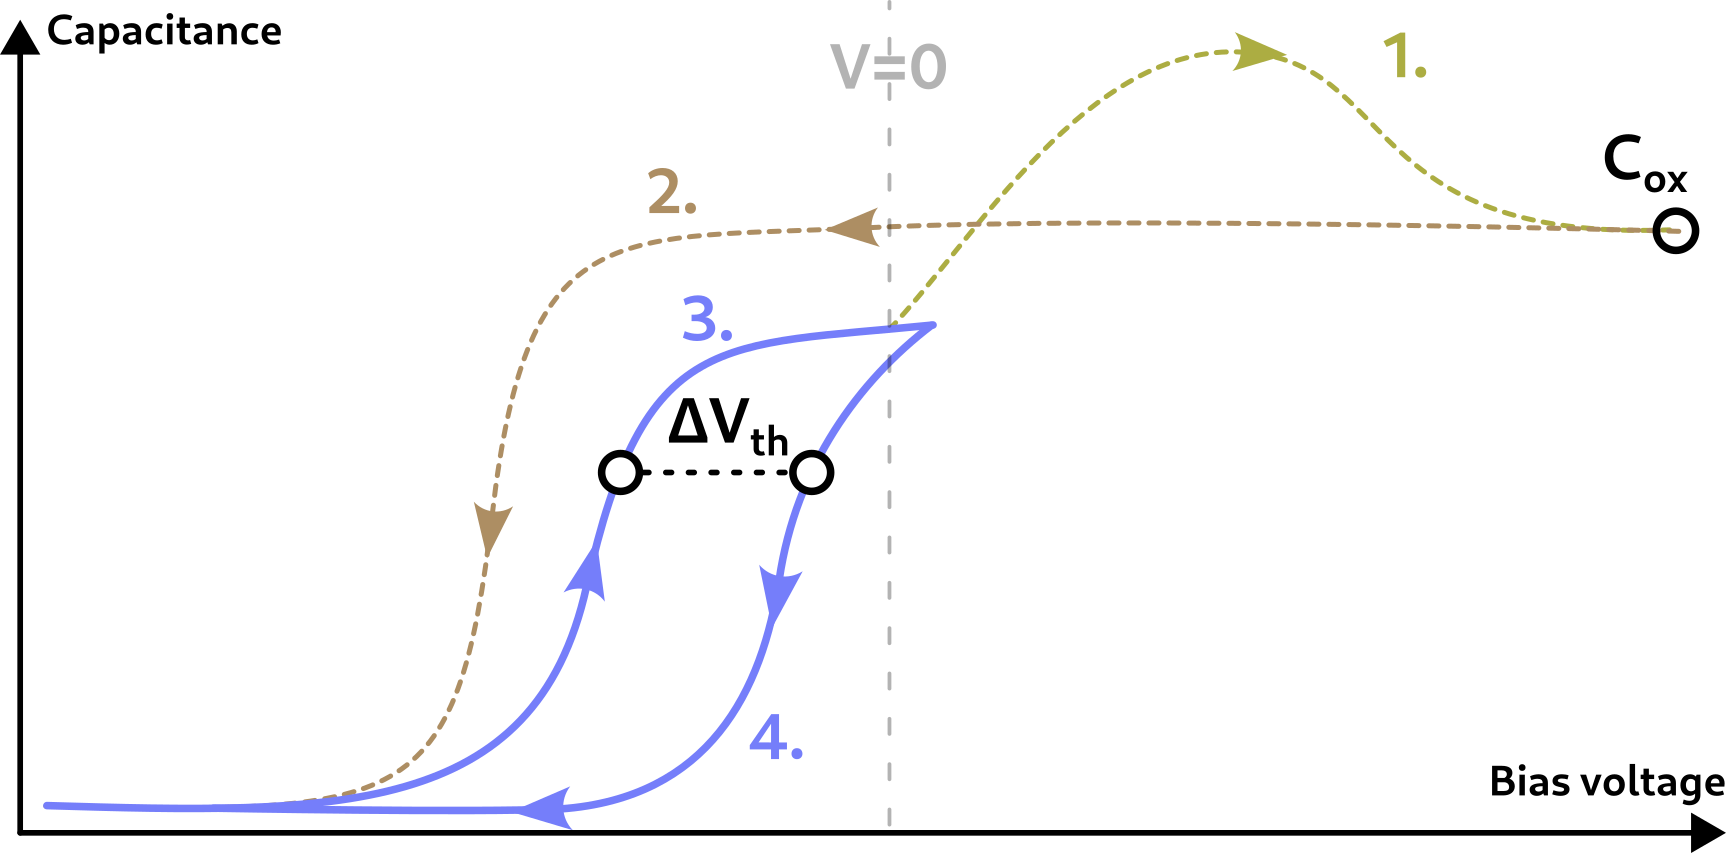
\includegraphics[width=0.70\textwidth]{fig/img/UniCV.png}
    \caption{Schematic illustration of the CV measurement schema with the
    desired values of $C_{ox}$ and $\Delta V_{th}$ clearly labeled. The schema
    is divided into 4 separate sweeps done in series where the device is initially
    polarized with a positive sweep to the maximum bias voltage (1) in order to
    find $C_{ox}$ followed by a negative sweep to polarize the device the opposite
    direction (2). To find $\Delta V_{th}$ two consecutive sweeps in opposite
    directions are done (3 and 4). A target voltage above $V=0$ but well below the coercive
    field is selected to induce the charge buildup without triggering the switching
    event. With these parameters measured one can calculate the defect density
    using equation \ref{eq:char_Vshift}.}
    \label{fig:char_CV}
\end{figure}

%%%%%%%%%%%%%%%%%%%%%%%%%%%
\chapter{Results and Analysis}\label{ch:res}

\section{Flashlamp Intensity and Film Temperature}
Crystallization of the hafnia films using the flash lamp annealing (FLA)
technique does not immediately reveal the temperature achieved in the films. Due
to the short time frames and the geometry of the FLA setup, one must simulate
the achieved temperature in the film from the structure of the samples and the
flash parameters. Flash duration and preheating temperature were set to
\SI{5}{\milli\second} and \SI{250}{\celsius} respectively in order to be below
the critical crystallization temperature before the FLA
flash \cite{migita2019phase}. Other simulation parameters are tabulated in
table \ref{tab:app_simparam} and produce figure \ref{fig:res_Comsol} showing the
resulting back and front peak temperature for different pulse energies. The figure also
includes pyrometer measurements of the back temperature during annealing
(green). The discrepancies on the order of \SI{20}{\kelvin} between simulated
back peak temperature (black) and the measured values are attributed to a 
lower reflectivity of the \ce{TiN} capping layer compared to the ideal values of
the simulation. Therefore, the model is deemed to be in reasonable agreement
with the experimental data and gives an estimate of the achieved surface peak temperature.

\begin{figure}[htbp]
    \centering
    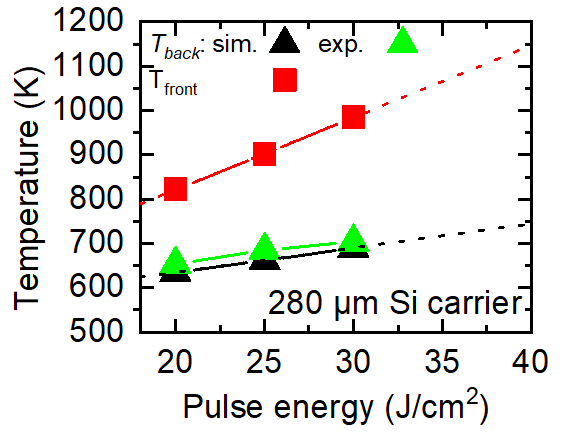
\includegraphics[width=.41\linewidth]{fig/img/COMSOLFlashInt.png}
    \caption{Simulated back and front peak temperatures of our samples using the
    simulation parameters tabulated in \ref{tab:app_simparam}. Pyrometer
    measurements of the back temperature measured during annealing (green) confirm
    the accuracy of these simulations.}\label{fig:res_Comsol}
\end{figure}

Figure~\ref{fig:res_Comsol} reveal a linear relationship between the pulse
energy ($E_{pulse}$) and the peak HZO film temperature ($T_{peak}$) for our
sample and FLA parameters (eq~\ref{eq:app_filmtemp}). This gives a more
convenient reference going forward using the achieved film temperature rather
than the pulse energy when describing different samples. The usually reported
crystallization temperature required to form the ferroelectric orthorhombic
phase of HZO is in the range of 400-\SI{600}{\celsius}
\cite{muller2012ferroelectricity, athle2022improved}.
The simulated peak surface temperatures in the
20-\SI{30}{\joule\per\square\centi\meter} pulse energy range are significantly
above this critical temperature and should therefore yield a sufficiently high
peak temperature to achieve ferroelectric properties in the HZO.

\section{Sample Specifications and Characterization}
As a reference point, samples were processed using rapid thermal processing
(RTP) as the annealing method in parallel to the FLA samples. These samples
proves as a point of comparison for the characterization of the FLA samples
throughout the work. The RTP samples were annealed at a temperature of
\SI{600}{\celsius} for 30 seconds. The electrical characterization of these
samples, as described in Chapter \ref{ch:char}, were measured and
tabulated in table \ref{tab:res_RTPref}. The remnant polarization and coercive
field are measured after a wakeup of $10^4$ cycles at a pulsing voltage of
\SI{3}{\volt}.

\begin{table}[htbp]
    \caption{Electrical characteristics for the RTP reference samples.}\label{tab:res_RTPref}
    \begin{tabular}{rlrl}
        \toprule
        \multicolumn{4}{c}{PUND, Endurance and Defect Density}\\\midrule
        Remnant Polarization & $P_r$ & $29.03 \pm 0.21$ &
        \si{\micro\coulomb\per\centi\meter\squared}\\
        Coercive Field & $E_c$ & $1.23 \pm 0.18$ &
        \si{\mega\volt\per\centi\meter}\\
        Endurance & & $23 \pm 11$ & $10^3$ cycles\\
        Defect Density & $D_d$ & $9.7 \pm 0.6$ &
        $10^{12}$ \si{\per\centi\meter\squared}
        \\\bottomrule
    \end{tabular}
\end{table}

The processing of the FLA samples are outlined in Section \ref{sec:FabProc}. For
the first FLA series, hereby denoted sample series 1, the flash intensity was
varied between 15-\SI{32.5}{\joule\per\centi\meter\squared} to reach different peak
temperatures in the film. The film deposition and annealing conditions for these
samples are summarized in table \ref{tab:app_IntC}.

Resulting electrical characterization from sample series 1 are shown in
figure \ref{fig:res_IntC}. As seen in figure \ref{fig:res_IntCPr} and
\ref{fig:res_IntCEc} the PUND characteristics show ferroelectric behaviour with
a strong dependence on peak film temperature. The onset of ferroelectricity for
these flashlamp annealed samples seem to be at a peak temperature between
550-\SI{630}{\celsius}. Therefore samples annealed with an intensity less than
\SI{25}{\joule/\centi\meter\squared} are omitted from some of the figures.
The remnant polarization and the coercive fields of these samples follow a similar
pattern reaching a peak of $20.12 \pm 0.59$ \si{\micro\coulomb\per\centi\meter\squared} and a
minimum of $1.46 \pm 0.14$ \si{\mega\volt\per\centi\meter} respectively at a peak
annealing temperature of \SI{711}{\celsius}. Higher temperature annealing
shows a degradation of these ferroelectric properties. The degradation could be
the effect of multiple factors such as thermal damage to the contacts or
further crystallization to the non-ferroelectric monoclinic phase but further
studies are needed to confirm these theories.

Figures \ref{fig:res_IntCPr} and \ref{fig:res_IntCEc} shows that the
described experimental process in Chapter \ref{ch:fab} is indeed a valid process for
fabricating ferroelectric capacitors of this caliber with comparable remnant
polarization and coercive fields to that of samples annealed through RTP.

\begin{figure}[htbp]
    \centering
    \begin{subfigure}{.4\linewidth}
        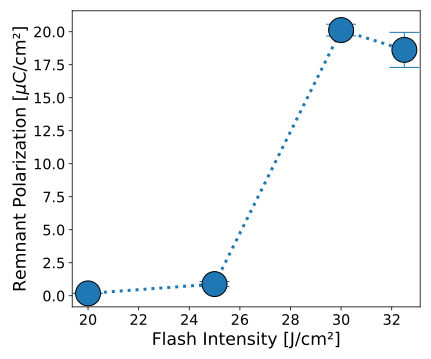
\includegraphics[width=\linewidth]{fig/FlashIntC_PrTrends.png}
        \caption{}\label{fig:res_IntCPr}
    \end{subfigure}
    \begin{subfigure}{.4\linewidth}
        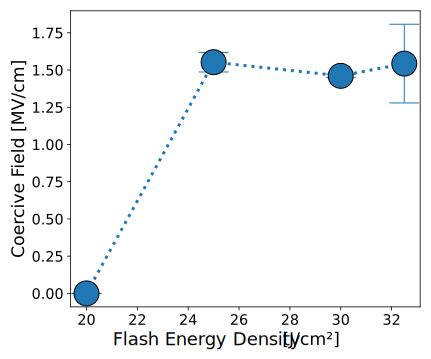
\includegraphics[width=\linewidth]{fig/FlashIntC_EcTrends.png}
        \caption{}\label{fig:res_IntCEc}
    \end{subfigure}
    \begin{subfigure}{.4\linewidth}
        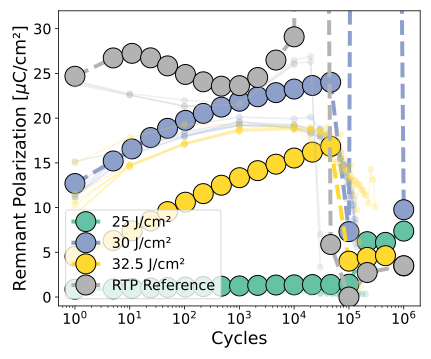
\includegraphics[width=\linewidth]{fig/FlashIntC_EnduTrends.png}
        \caption{}\label{fig:res_IntCEndu}
    \end{subfigure}
    \begin{subfigure}{.4\linewidth}
        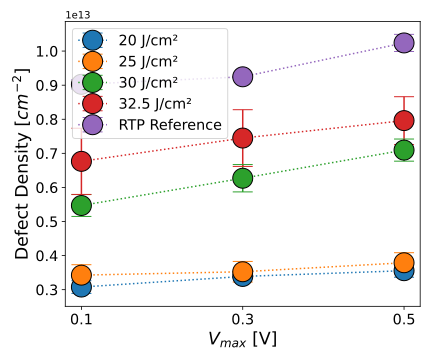
\includegraphics[width=\linewidth]{fig/FlashIntC_DDTrends.png}
        \caption{}\label{fig:res_IntCDD}
    \end{subfigure}
    \caption{Plotted data from sample series 1. Figures a and
        b show the ferroelectric response of the samples at varying peak
        annealing temperature indicating comparable ferroelectric response to
        the RTP annealed samples presented in table \ref{tab:res_RTPref}.
        Figure c and d show improved endurance and reduced defect density
        respectively for all samples annealed through FLA compared to the RTP
        sample.}\label{fig:res_IntC}
\end{figure}

Furthermore, figure \ref{fig:res_IntCEndu} show an increased endurance for
sample series 1 compared to the RTP reference. The comparable sample 4 flashed
with \SI{30}{\joule\per\centi\meter\squared} had a endurance roughly 6 times
greater at values in the range $(127 \pm 13)$ $\cdot 10^3$ cycles. The barely
ferroelectric sample 3 flashed at \SI{25}{\joule\per\centi\meter\squared}
did not breakdown before the measurements ended at $200$ $\cdot 10^3$ cycles and
the endurance of these capacitors should be investigated further to reach a
conclusion for their viability for use in certain gate stacks \cite{dawber2005physics}.
Similarly to $P_r$ and $E_c$, annealing at a higher peak temperature results in degraded
endurance to a value of $(82 \pm 46)$ $\cdot 10^3$ cycles. These values however
are still an improvement compared to the RTP sample.

The improved endurance could be a result of the reduced defect density of the
flash lamp annealed films as shown in figure \ref{fig:res_IntCDD} using the
method described in section \ref{sec:CV}. The measurements reveal a defect
reduction of up to a factor of 3 for sample 3 and close to a factor of 2 for
sample showing comparable $P_r$ and $E_c$ to the RTP sample. This is likely due
to the reduced thermal budget for the FLA samples which generates less initial
defects during the annealing step. However, after sufficiently many cycles the
generated defects (vacancies) start to collect at the \ce{HZO} grain boundaries
increasing the leakage through the oxide and causes the breakdown. However,
the data studied here is not enough to rigorously conclude these theories
\cite{pesic2016physical, athle2022improved}. See table \ref{tab:res_series1} for
a summary of the attained values.

\begin{table}[htbp]
    \caption{Electrical characteristics for sample 4 in sample series
    1. See table \ref{tab:app_IntC} for processing conditions.}\label{tab:res_series1}
    \begin{tabular}{rlrl}
        \toprule
        \multicolumn{4}{c}{PUND, Endurance and Defect Density}\\\midrule
        Remnant Polarization & $P_r$ & $20.12 \pm 0.59$ &
        \si{\micro\coulomb\per\centi\meter\squared}\\
        Coercive Field & $E_c$ & $1.46 \pm 0.14$ & \si{\mega\volt\per\centi\meter}\\
        Endurance & & $127 \pm 13$ & $10^3$ cycles\\
        Defect Density & $D_d$ & $6.1 \pm 0.7$ & $10^{12}$
        \si{\per\centi\meter\squared}
        \\\bottomrule
    \end{tabular}
\end{table}

Although sample series 1 resulted in improved endurance and lower defect density
along with comparable PUND data to the RTP samples, the peak annealing
temperature is still to high in order to significantly reduce the amount of
defects in the film. A closer look at figure \ref{fig:res_IntCDD} and the barely
ferroelectric sample 3 annealed at a flash intensity of
\SI{25}{\joule\per\centi\meter\squared} reveal a further reduction of the defect
density at the cost of ferroelectric response (figure \ref{fig:res_IntCPr}).
Maintaining that low peak annealing temperature over multiple flashes could
result in improved PUND data while not inducing additional defects.

For sample series 2 and 3, tabulated in table \ref{tab:app_NumA} and
\ref{tab:app_NumC} respectively, the number of flashes were varied up to a
maximum of 8 flashes for two different peak annealing temperatures at the onset
of crystallization. The flashes were manually timed at an interval of
approximately \SI{200}{\second}.

Resulting electrical characteristics of sample series 2 and 3 are shown in
figures \ref{fig:res_NumACPUND} and \ref{fig:res_NumACEnduDD}. Figure
\ref{fig:res_NumACPr} reveal an increased ferroelectric response with
additional flashes up to a maximum of $22.98 \pm 1.02$
\si{\micro\coulomb\per\centi\meter\squared} for sample series 2. Sample series 3
on the other hand is not annealed to a significantly high peak temperature to
achieve ferroelectricity until 8 flashes; but even then not to a significant
degree. Sample series 2 show a similar degradation of the ferroelectric response
when flashing up to 8 times as with the increased flash intensity in figure
\ref{fig:res_IntCPr} where again further studies are needed to confirm its
causes. The achieved coercive field as shown in figure \ref{fig:res_NumACEc}
is comparable with both sample series 1 and the RTP sample.

\begin{figure}[htbp]
    \centering
    \begin{subfigure}{.4\linewidth}
        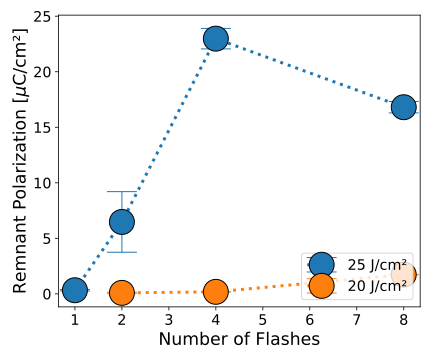
\includegraphics[width=\linewidth]{fig/FlashNumA+C_PrTrends.png}
        \caption{}\label{fig:res_NumACPr}
    \end{subfigure}
    \begin{subfigure}{.4\linewidth}
        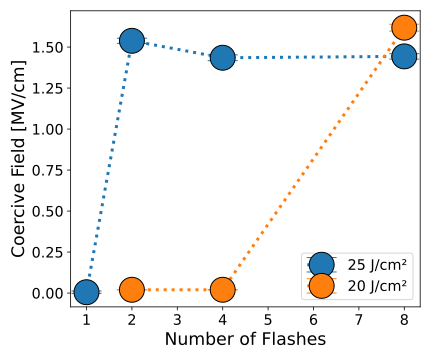
\includegraphics[width=\linewidth]{fig/FlashNumA+C_EcTrends.png}
        \caption{}\label{fig:res_NumACEc}    
    \end{subfigure}
    \caption{Plotted PUND data from sample series 2 and 3. Figure a and b show the
    evolution of the remnant polarization and the coercive field respectively
    over varying number of flashes for two different peak annealing temperatures.
    Increasing the number of flashes with reduced peak annealing temperature
    results in comparable ferroelectric response to the RTP sample as tabulated
    in table \ref{tab:res_RTPref}.}\label{fig:res_NumACPUND}
\end{figure}

Similarly to sample series 1, figure \ref{fig:res_NumACEnduDD} show increased
endurance as well as a lower defect density compared to the RTP sample. Sample 4
of sample series 2 which has the most similar ferroelectric response to the RTP
sample had an endurance in the range $(53 \pm 11)$ $\cdot 10^3$ cycles; an
improvement of a factor of 2. Other samples in the same series showed longer
endurances but at the cost of remnant polarization. More interestingly, the
defect density of sample series 2 shown in figure \ref{fig:res_NumADD} does
increase with multiple flashes reaching a saturated value at 4 flashes an
beyond. This gives indication for the peak annealing temperature of
\SI{630}{\celsius} still being to high in order to avoid the diffusion of
defects in the samples. After 4 flashes the defect density reaches a saturated
value where additional flashes only affects the already generated defects and
assists in the pinning of the domains lowering $P_r$ as shown in figure
\ref{fig:res_IntCPr}.

Sample series 3 does not give any ferroelectric response until the 8th flash as
shown in figure \ref{fig:res_NumACPr}. This is likely due to the low total
thermal impact of the \SI{5}{\milli\second} pulses at this peak annealing
temperature. However, as indicated by figure \ref{fig:res_NumCDD}, the defect
density of these samples also increase with additional flashes, reaching
approximately the same value as for sample series 2 but showing a significantly
lower ferroelectric response. This implies the total energy deposited in the
samples during flashing is enough to induce additional defects but barely enough
to crystallize the HZO to the orthorhombic phase. See table
\ref{tab:res_series2} for a summary of the attained values for sample series 2.

\begin{figure}[htbp]
    \centering
    \begin{subfigure}{.4\linewidth}
        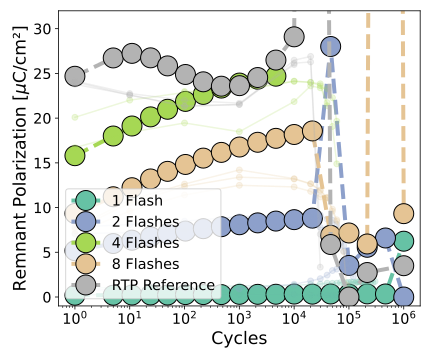
\includegraphics[width=\linewidth]{fig/FlashNumA_EnduTrends.png}
        \caption{}\label{fig:res_NumAEndu}
    \end{subfigure}
    \begin{subfigure}{.4\linewidth}
        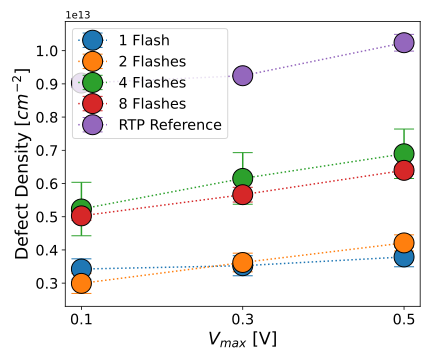
\includegraphics[width=\linewidth]{fig/FlashNumA_DDTrends.png}
        \caption{}\label{fig:res_NumADD}
    \end{subfigure}
    \begin{subfigure}{.4\linewidth}
        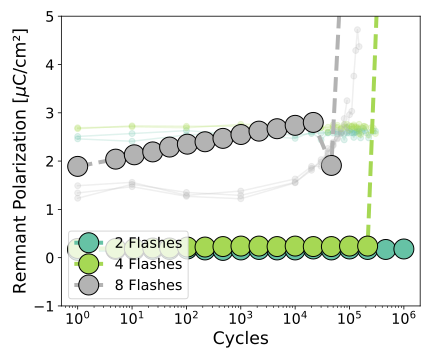
\includegraphics[width=\linewidth]{fig/FlashNumC_EnduTrends.png}
        \caption{}\label{fig:res_NumCEndu}
    \end{subfigure}
    \begin{subfigure}{.4\linewidth}
        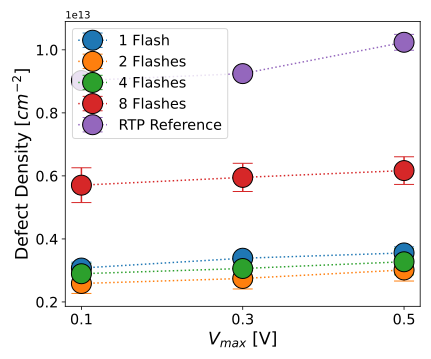
\includegraphics[width=\linewidth]{fig/FlashNumC_DDTrends.png}
        \caption{}\label{fig:res_NumCDD}    
    \end{subfigure}
    \caption{Plotted endurance and defect density from sample series
    2 and 3. Figures a and b show the data from samples series 2 while
    figures c and d show the data from sample series
    3. Increasing the number of flashes with reduced peak annealing temperature
    affects the defect density up to a point where additional flashes only assists
    in pinning the ferroelectric domains. The measured endurance of these samples
    are greater compared to the RTP samples.}\label{fig:res_NumACEnduDD}
\end{figure}

\begin{table}[htbp]
    \caption{Electrical characteristics for sample 3 in sample series
    2. See table \ref{tab:app_NumA} for processing
    conditions.}\label{tab:res_series2}
    \begin{tabular}{rlrl}
        \toprule
        \multicolumn{4}{c}{PUND, Endurance and Defect Density}\\\midrule
        Remnant Polarization & $P_r$ & $22.98 \pm 1.02$ &
        \si{\micro\coulomb\per\centi\meter\squared}\\
        Coercive Field & $E_c$ & $1.44 \pm 0.36$ & \si{\mega\volt\per\centi\meter}\\
        Endurance & & $53 \pm 11$ & $10^3$ cycles\\
        Defect Density & $D_d$ & $5.9 \pm 1.1$ & $10^{12}$
        \si{\per\centi\meter\squared}
        \\\bottomrule
    \end{tabular}
\end{table}

Sample series 1 through 3 show only slight performance improvements to the RTP
samples due to the flash intensity being to high to facilitate additional
crystallization before inducing other effects or the time required for multiple
flashes attributing to an increased defect density without further
crystallization. Both these effects contribute to increased domain pinning and
eventually the breakdown of the individual capacitors. In an effort to minimize the
energy needed during annealing, the ALD temperature could be increased to
potentially pre-crystallize the HZO during growth, hopefully resulting in a
lower thermal budget needed in the annealing step.

For sample series 4 and 5, tabulated in table \ref{tab:app_IntE} and
\ref{tab:app_NumD} respectively, the growth temperature during annealing was
increased from \SI{200}{\celsius} to \SI{270}{\celsius}. The HZO growth per
cycle at this elevated temperature is reduced by roughly \SI{20}{\percent} in
our equipment. To compensate for the lower growth per cycle the amount of cycles
was increased to 60:60 to maintain the same HZO thickness as previous samples.

The plotted data from sample series 4 is shown in figure \ref{fig:res_IntE}. The
increased growth temperature does indeed reduce the peak annealing temperature
required to reach the onset of ferroelectricity in the samples as shown in
figure \ref{fig:res_IntEPr}. With the increased growth temperature the window in
which a significant ferroelectric response is achieved is widened and a reduced
coercive field is noted in figure \ref{fig:res_IntEEc}. However, with our
selected peak annealing temperatures it is not clear whether we have surpassed
or yet to have reached the saturation point as noted at a growth temperature of
\SI{200}{\celsius}. It would be interesting to increase the peak annealing
temperature further to see the effects of a higher temperature anneal on the
ferroelectric response.

\begin{figure}[htbp]
    \centering
    \begin{subfigure}{.4\linewidth}
        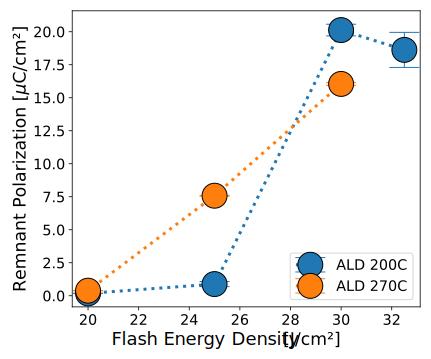
\includegraphics[width=\linewidth]{fig/FlashIntC+E_PrTrends.png}
        \caption{}\label{fig:res_IntEPr}
    \end{subfigure}
    \begin{subfigure}{.4\linewidth}
        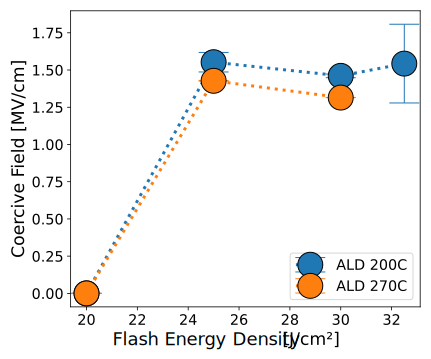
\includegraphics[width=\linewidth]{fig/FlashIntC+E_EcTrends.png}
        \caption{}\label{fig:res_IntEEc}
    \end{subfigure}
    \begin{subfigure}{.4\linewidth}
        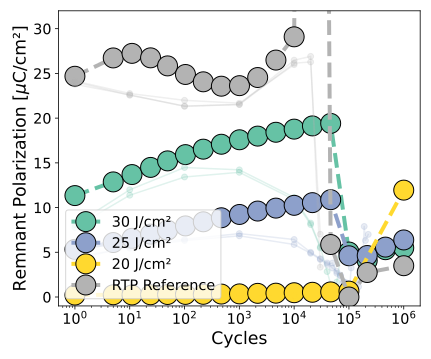
\includegraphics[width=\linewidth]{fig/FlashIntE_EnduTrends.png}
        \caption{}\label{fig:res_IntEEndu}
    \end{subfigure}
    \begin{subfigure}{.4\linewidth}
        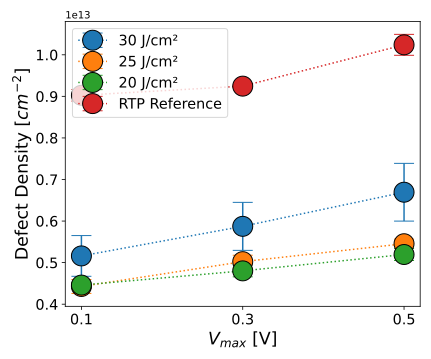
\includegraphics[width=\linewidth]{fig/FlashIntE_DDTrends.png}
        \caption{}\label{fig:res_IntEDD}    
    \end{subfigure}
    \caption{Plotted data from sample series 4. Figures a and b show the
    ferroelectric response of samples grown at different ALD temperatures for
    varying peak annealing temperatures indicating that increasing growth
    temperature assists in lowering the required temperature to reach the onset of
    ferroelectricity. Figure c show improved endurance compared to the RTP
    sample. Figure d shows an overall increase in defect density for samples grown
    at elevated temperature but also a reduced impact of the annealing step on
    defect generation.}\label{fig:res_IntE}
\end{figure}

The endurance of these samples show similar improvement as earlier FLA treated
samples, as seen in figure \ref{fig:res_IntEEndu}. With improvements up to a
factor of five with comparable $P_r$ while samples without significant
ferroelectric response do not reach breakdown $\leq 300\cdot10^3$ cycles. The
increased endurance shows in figure \ref{fig:res_IntEDD} as well through the
reduced defect density of these samples. Interestingly, for these samples an
overall increase in defect density is seen even for samples which do not show
any ferroelectric response. Increasing the peak annealing temperature seem to
have a reduced impact on defect generation and is ultimately comparable with
previous FLA treated samples at a peak annealing temperature of
\SI{711}{\celsius}. This revelation seem to show that the defect generation is
energy dependant and that defects that would be generated by the one
\SI{30}{\joule\per\centi\meter\squared} are being generated during growth
instead. With many defects already generated during growth, the peak annealing
temperature is not high enough to induce additional defects. See table
\ref{tab:res_series4} for a summary of the measured values.

\begin{table}[htbp]
    \caption{Electrical characteristics for sample 3 in sample series
    4. See table \ref{tab:app_IntE} for processing
    conditions.}\label{tab:res_series4}
    \begin{tabular}{rlrl}
        \toprule
        \multicolumn{4}{c}{PUND, Endurance and Defect Density}\\\midrule
        Remnant Polarization & $P_r$ & $16.05 \pm 0.63$ &
        \si{\micro\coulomb\per\centi\meter\squared}\\
        Coercive Field & $E_c$ & $1.32 \pm 0.13$ & \si{\mega\volt\per\centi\meter}\\
        Endurance & & $50 \pm 28$ & $10^3$ cycles\\
        Defect Density & $D_d$ & $5.8 \pm 0.7$ & $10^{12}$
        \si{\per\centi\meter\squared}
        \\\bottomrule
    \end{tabular}
\end{table}

Sample series 4 showed that increasing growth temperature assisted in lowering
the required peak annealing temperature to reach the onset of ferroelectricity
in addition to a reduced impact on defect generation during annealing. However,
to reach significant values of remnant polarization a high peak annealing
temperature is still required. Using the knowledge from sample series 2 and 3 it
might be possible to reduce the impact of annealing on defect generation even
further. 

\begin{figure}[htbp]
    \centering
    \begin{subfigure}{.4\linewidth}
        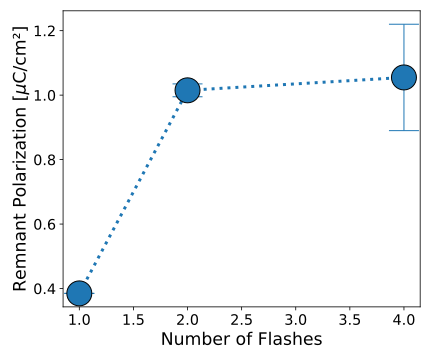
\includegraphics[width=\linewidth]{fig/FlashNumD_PrTrends.png}
        \caption{}\label{fig:res_NumDPr}
    \end{subfigure}
    \begin{subfigure}{.4\linewidth}
        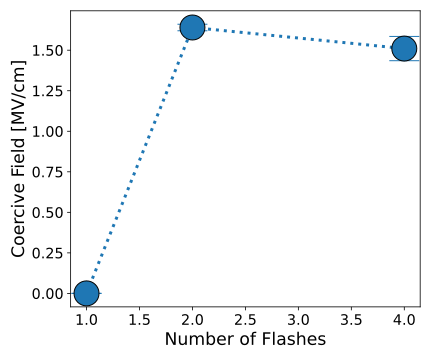
\includegraphics[width=\linewidth]{fig/FlashNumD_EcTrends.png}
        \caption{}\label{fig:res_NumDEc}
    \end{subfigure}
    \begin{subfigure}{.4\linewidth}
        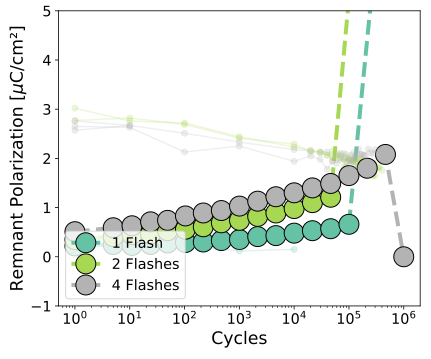
\includegraphics[width=\linewidth]{fig/FlashNumD_EnduTrends.png}
        \caption{}\label{fig:res_NumDEndu}
    \end{subfigure}
    \begin{subfigure}{.4\linewidth}
        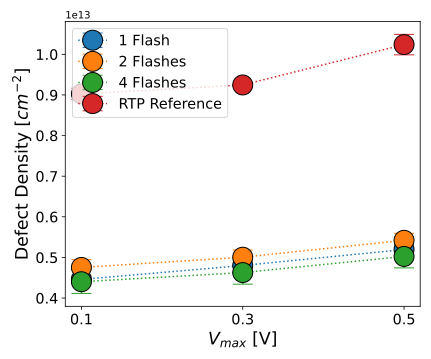
\includegraphics[width=\linewidth]{fig/FlashNumD_DDTrends.png}
        \caption{}\label{fig:res_NumDDD}    
    \end{subfigure}
    \caption{Plotted data from sample series 5. Figures a and b show the
    ferroelectric response of the samples annealed at a peak annealing
    temperature of \SI{548}{\celsius} over varying number of flashes. The figures
    reveal that the temperature is not high enough to reach the onset of
    ferroelectricity despite having been grown at an elevated ALD temperature.
    Figure c shows the supposed endurance that is only affects by the increasing
    leakage current during cycling. Figure d affirms the higher defect density of
    samples grown at the elevated growth temperature and shown no effect on defect
    generation throughout the annealing steps.}\label{fig:res_NumD}
\end{figure}

The plotted data from sample series 5 is shown in figure \ref{fig:res_NumD}. The
peak annealing temperature for these samples are \SI{548}{\celsius} in the
attempt to incrementally reach the onset of ferroelectricity with additional
flashes. Figures \ref{fig:res_NumDPr} and \ref{fig:res_NumDEc} show $P_r$ and
$E_c$ respectively and reveal that the peak annealing temperature is not
sufficient to reach the onset of ferroelectricity for up to 4 flashes. Although
some response is measured for all samples, this is attributed to the noisiness
of non-ferroelectric samples. Since the samples are not ferroelectric, the
endurance in figure \ref{fig:res_NumDEndu} show only an increasing remnant
polarization response due to increased leakage current during cycling. Figure
\ref{fig:res_NumDDD} show the same elevated defect density as in figure
\ref{fig:res_IntEDD} which stay consistent throughout annealing.

%%%%%%%%%%%%%%%%%%%%%%%%%%
\chapter{Conclussion}\label{chap:conc}

This report shows successful integration of ferroelectric HZO into a
\ce{InAs}/\ce{HZO}/\ce{TiN} stack using a flash lamp annealing (FLA) technique. The
resulting capacitors show comparable ferroelectric response with capacitors
annealed through rapid thermal processing (RTP) with an improved endurance up
to a factor 5. The improved endurance is attributed to the reduced defect
density of the films processed using FLA. This in part due to the reduced
thermal budget of the FLA technique which reduces the diffusion of oxygen
vacancies as well as the formation of \ce{As} and \ce{In} oxides from the
substrate \cite{kang2016structural}. The reduced defect density allows for
additional endurance cycling before breakdown of the ferroelectric capacitor.

In our efforts of further reducing the defect density, both multiple flashes at
a lower peak annealing temperature and pre-crystallization during growth was
examined. However, these efforts showed varied success. Additional flashes
showed only marginal improvements up to the amount of flashes tested during
these experiments. Using a flash lamp annealer which can produce multiple
flashes at a higher repetition rate could prove fruitful. Pre-crystallization
of the HZO during growth showed marginal success in lowering the required peak
annealing temperature to reach the onset of ferroelectricity but did in itself
prove detrimental to the defect density of the samples.

In order to better understand the material effects of these efforts this data
could be combined with studies of the oxide bulk and surface to identify
defects and their properties. In a complementary study by R. Athle et al the
data from this study is combined with XPS data to better understand the
defects of the samples \cite{athle2022improved}.

%%%%%%%%%%%%%%%%%%%%%%%%%%%%%%%%%%%%%%%
%% References
\bibliography{Exjobbreport.bib}
\bibliographystyle{ieeetr}


%%%%%%%%%%%%%%%%%%
\appendix
%%%%%%%%%%%%%%%%%%%
\chapter{Extra Material}\label{app:extra}
\begin{table}[htbp]
    \centering
    \caption{Relevant simulation parameters used in COMSOL to achieve
    figure~\ref{fig:res_Comsol}. The \ce{InAs/HZO/TiN} is part of the sample
while \ce{Si} is a carrier wafer part of the FLA experimental setup.}\label{tab:app_simparam}
    \begin{tabular}{crcc}
        \toprule
        Layer & Thickness & Doping & Reflectivity \\\midrule
        \ce{TiN} & \SI{10}{\nano\meter} &~- & 0.41 \\ 
        \ce{HZO} & \SI{10}{\nano\meter} & 1:1 (\ce{Hf/Zr}) &~- \\ 
        \ce{InAs} & \SI{280}{\micro\meter} & \SI{1e16}{\per\centi\meter\tothe{3}} &~- \\ 
        \ce{Si} & \SI{280}{\micro\meter} &~- &~- \\\bottomrule
    \end{tabular}
\end{table}

\begin{equation}\label{eq:app_filmtemp}
    T_{peak} [\si{\kelvin}] = 495.5 + 16.3 \cdot E_{pulse} [\si{\joule\per\square\centi\meter}]
\end{equation}

\chapter{Processing Parameters}\label{app:procparam}
\begin{table}[htbp]
    \caption{Selected processing conditions for sample series 1.}\label{tab:app_IntC}
    \begin{tabular}{rlccccc}
        \toprule
        \multicolumn{2}{l}{Sample Number} & 1 & 2 & 3 & 4 & 5 \\\midrule
        \multicolumn{1}{c}{HZO} & & & & & & \\
        Growth Temperature & [\si{\celsius}] & 200 & 200 & 200 & 200 & 200 \\
        Deposition Cycles & [\ce{Hf}:\ce{Zr}] & 50:50 & 50:50 & 50:50 & 50:50 & 50:50 \\\midrule
        \multicolumn{1}{c}{FLA} & & & & & & \\
        Preheat Temperature & [\si{\celsius}] & 250 & 250 & 250 & 250 & 250 \\
        Peak Temperature & [\si{\celsius}] & \textbf{467} & 
        \textbf{548} & \textbf{630} & \textbf{711} & \textbf{752} \\
        Number of Flashes & & 1 & 1 & 1 & 1 & 1 \\\bottomrule
    \end{tabular}
\end{table}

\begin{table}[htbp]
    \caption{Selected processing conditions for sample series
    2.}\label{tab:app_NumA}
    \begin{tabular}{rlcccc}
        \toprule
        \multicolumn{2}{l}{Sample Number} & 1 & 2 & 3 & 4 \\\midrule
        \multicolumn{1}{c}{HZO} & & & & & & \\
        Growth Temperature & [\si{\celsius}] & 200 & 200 & 200 & 200 \\
        Deposition Cycles & [\ce{Hf}:\ce{Zr}] & 50:50 & 50:50 & 50:50 & 50:50 \\\midrule
        \multicolumn{1}{c}{FLA} & & & & & \\
        Preheat Temperature & [\si{\celsius}] & 250 & 250 & 250 & 250 \\
        Peak Temperature & [\si{\celsius}] & 630 & 630 & 630 & 630 \\
        Number of Flashes & & \textbf{1} & \textbf{2} & \textbf{4} & \textbf{8} \\\bottomrule
    \end{tabular}
\end{table}

\begin{table}[htbp]
    \caption{Selected processing conditions for sample series
    3.}\label{tab:app_NumC}
    \begin{tabular}{rlccc}
        \toprule
        \multicolumn{2}{l}{Sample Number} & 1 & 2 & 3 \\\midrule
        \multicolumn{1}{c}{HZO} & & & & \\
        Growth Temperature & [\si{\celsius}] & 200 & 200 & 200 \\
        Deposition Cycles & [\ce{Hf}:\ce{Zr}] & 50:50 & 50:50 & 50:50 \\\midrule
        \multicolumn{1}{c}{FLA} & & & & \\
        Preheat Temperature & [\si{\celsius}] & 250 & 250 & 250 \\
        Peak Temperature & [\si{\celsius}] & 548 & 548 & 548 \\
        Number of Flashes & & \textbf{2} & \textbf{4} & \textbf{8} \\\bottomrule
    \end{tabular}
\end{table}

\begin{table}[htbp]
    \caption{Selected processing conditions for sample series
    4.}\label{tab:app_IntE}
    \begin{tabular}{rlccc}
        \toprule
        \multicolumn{2}{l}{Sample Number} & 1 & 2 & 3 \\\midrule
        \multicolumn{1}{c}{HZO} & & & & \\
        Growth Temperature & [\si{\celsius}] & 270 & 270 & 270 \\
        Deposition Cycles & [\ce{Hf}:\ce{Zr}] & 60:60 & 60:60 & 60:60 \\\midrule
        \multicolumn{1}{c}{FLA} & & & & \\
        Preheat Temperature & [\si{\celsius}] & 250 & 250 & 250 \\
        Peak Temperature & [\si{\celsius}] & \textbf{548} & \textbf{630} &
        \textbf{711} \\
        Number of Flashes & & 1 & 1 & 1 \\\bottomrule
    \end{tabular}
\end{table}

\begin{table}[htbp]
    \caption{Selected processing conditions for sample series
    5.}\label{tab:app_NumD}
    \begin{tabular}{rlccc}
        \toprule
        \multicolumn{2}{l}{Sample Number} & 1 & 2 & 3 \\\midrule
        \multicolumn{1}{c}{HZO} & & & & \\
        Growth Temperature & [\si{\celsius}] & 270 & 270 & 270 \\
        Deposition Cycles & [\ce{Hf}:\ce{Zr}] & 60:60 & 60:60 & 60:60 \\\midrule
        \multicolumn{1}{c}{FLA} & & & & \\
        Preheat Temperature & [\si{\celsius}] & 250 & 250 & 250 \\
        Peak Temperature & [\si{\celsius}] & 548 & 548 & 548 \\
        Number of Flashes & & \textbf{1} & \textbf{2} & \textbf{4} \\\bottomrule
    \end{tabular}
\end{table}

\end{document}
